\documentclass[a4paper,12pt]{article}
\usepackage[utf8]{inputenc}
\usepackage{amsmath}
\usepackage{amsfonts}
\usepackage{amssymb}

\usepackage[T1]{fontenc}
\usepackage{gensymb}
\usepackage[hidelinks]{hyperref}
\usepackage{lmodern}
\usepackage{longtable}
\usepackage{booktabs}
\usepackage{array}
\usepackage{tabularx}
\usepackage{titlesec}
\usepackage{indentfirst}
\usepackage{float}
\usepackage{graphicx}

\usepackage{xcolor}


\usepackage[left=2cm,right=2cm,top=2cm,bottom=2cm]{geometry}

\usepackage[numbers]{natbib}


\titleformat{\section}{\large\bfseries}{\thesection}{1em}{}

\author{Adelynn Shirts}
\title{Obesity Classification with and without Weight Features}
\date{}
\begin{document}

\maketitle
\section{Introduction}

Understanding and predicting obesity levels is a critical aspect of public health. With obesity rates in the United States on the rise since the early 2000s, it has become essential to carefully monitor this health crisis. In this project, I used data from the UCI Obesity Level Estimation dataset to build models to classify participants as Obese or not based on their lifestyle and demographics.

My goal was to train and evaluate several models to identify the most effective approach to classifying obesity status. I used balanced accuracy as my primary evaluation metric, as the data is slightly imbalanced, but other key metrics, like the AUC and confusion matrices, were also calculated. I also explored feature importance across different models to understand which factors contribute most to obesity.
\section{Data}
The dataset is comprised of 2111 observations and contains both numerical and categorical variables regarding lifestyle and demographics. The original target variable, Nobeyesdad, contained 7 categories ranging from underweight to type 3 obesity. I collapsed the target into a binary response variable where: 
$0 =$ Not Obese (Insufficient Weight, Normal Weight, Overweight I, Overweight II) and
$1 =$ Obese (Obesity I, Obesity II, Obesity III).

The final dataset included variables that cover gender, age, height, weight, and various eating and lifestyle habits. I also converted categorical variables to numeric encodings summarized in the table below. As some of the models require scaled inputs, the data was then standardized. 

\begin{table}[H]
\centering
\footnotesize
\begin{tabular}{>{\raggedright\arraybackslash}p{3.5cm} >{\raggedright\arraybackslash}p{5.5cm} >{\raggedright\arraybackslash}p{4.2cm}}
\toprule
\textbf{Variable} & \textbf{Original Values} & \textbf{Numeric Encoding} \\
\midrule
Gender & Male, Female & Male = 0, Female = 1 \\
family\_history\_
with\_overweight & no, yes & no = 0, yes = 1 \\
FAVC & no, yes & no = 0, yes = 1 \\
SMOKE & no, yes & no = 0, yes = 1 \\
SCC & no, yes & no = 0, yes = 1 \\
CAEC & no, Sometimes, Frequently, Always & 0 = no, 1 = Sometimes, 2 = Frequently, 3 = Always \\
CALC & no, Sometimes, Frequently, Always & 0 = no, 1 = Sometimes, 2 = Frequently, 3 = Always \\
MTRANS & Public\_Transportation, Automobile, Walking, Motorbike, Bike & 0 = Public\_Transportation, 1 = Automobile, 2 = Walking, 3 = Motorbike, 4 = Bike \\
\bottomrule
\end{tabular}
\caption{Encodings for categorical variables}
\label{tab:encodings}
\end{table}

\section{Preliminary Data Analysis and Visualizations}

After standardizing the data, I calculated some basic summary statistics to get a better idea of the distributions of the data. I further made histograms to model the numeric data and bar charts for the categorical features, as seen below.

\begin{figure}[H]
    \centering
    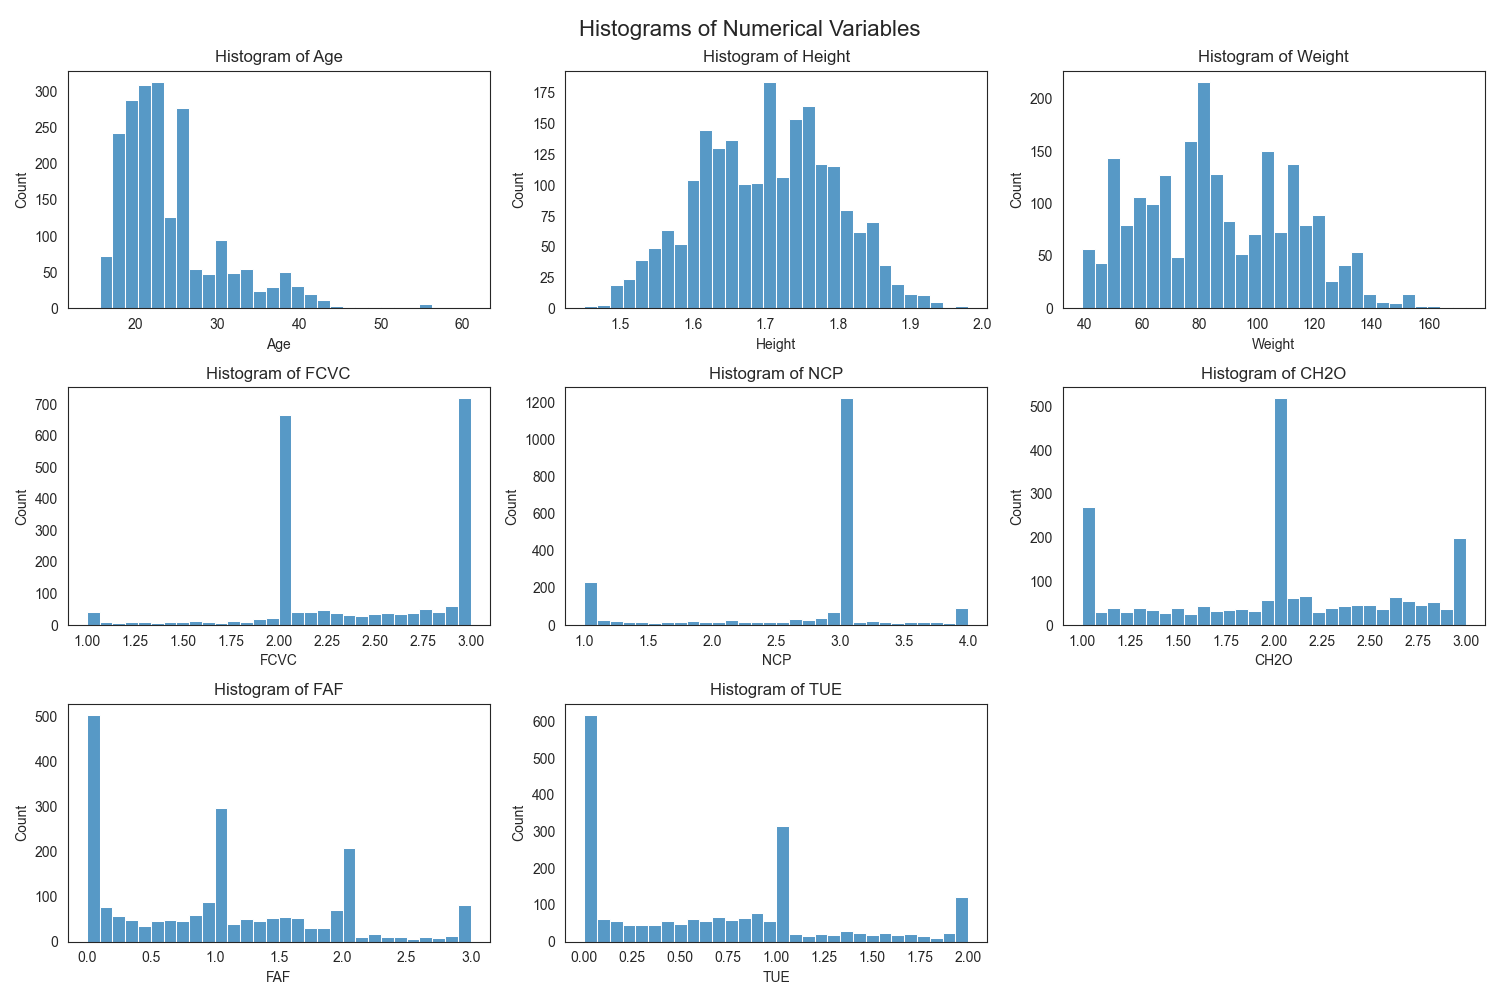
\includegraphics[width=0.8\textwidth]{Histograms.png}
    \caption{Histograms of numerical variables}
    \label{fig:histograms}
\end{figure}

\begin{figure}[H]
    \centering
    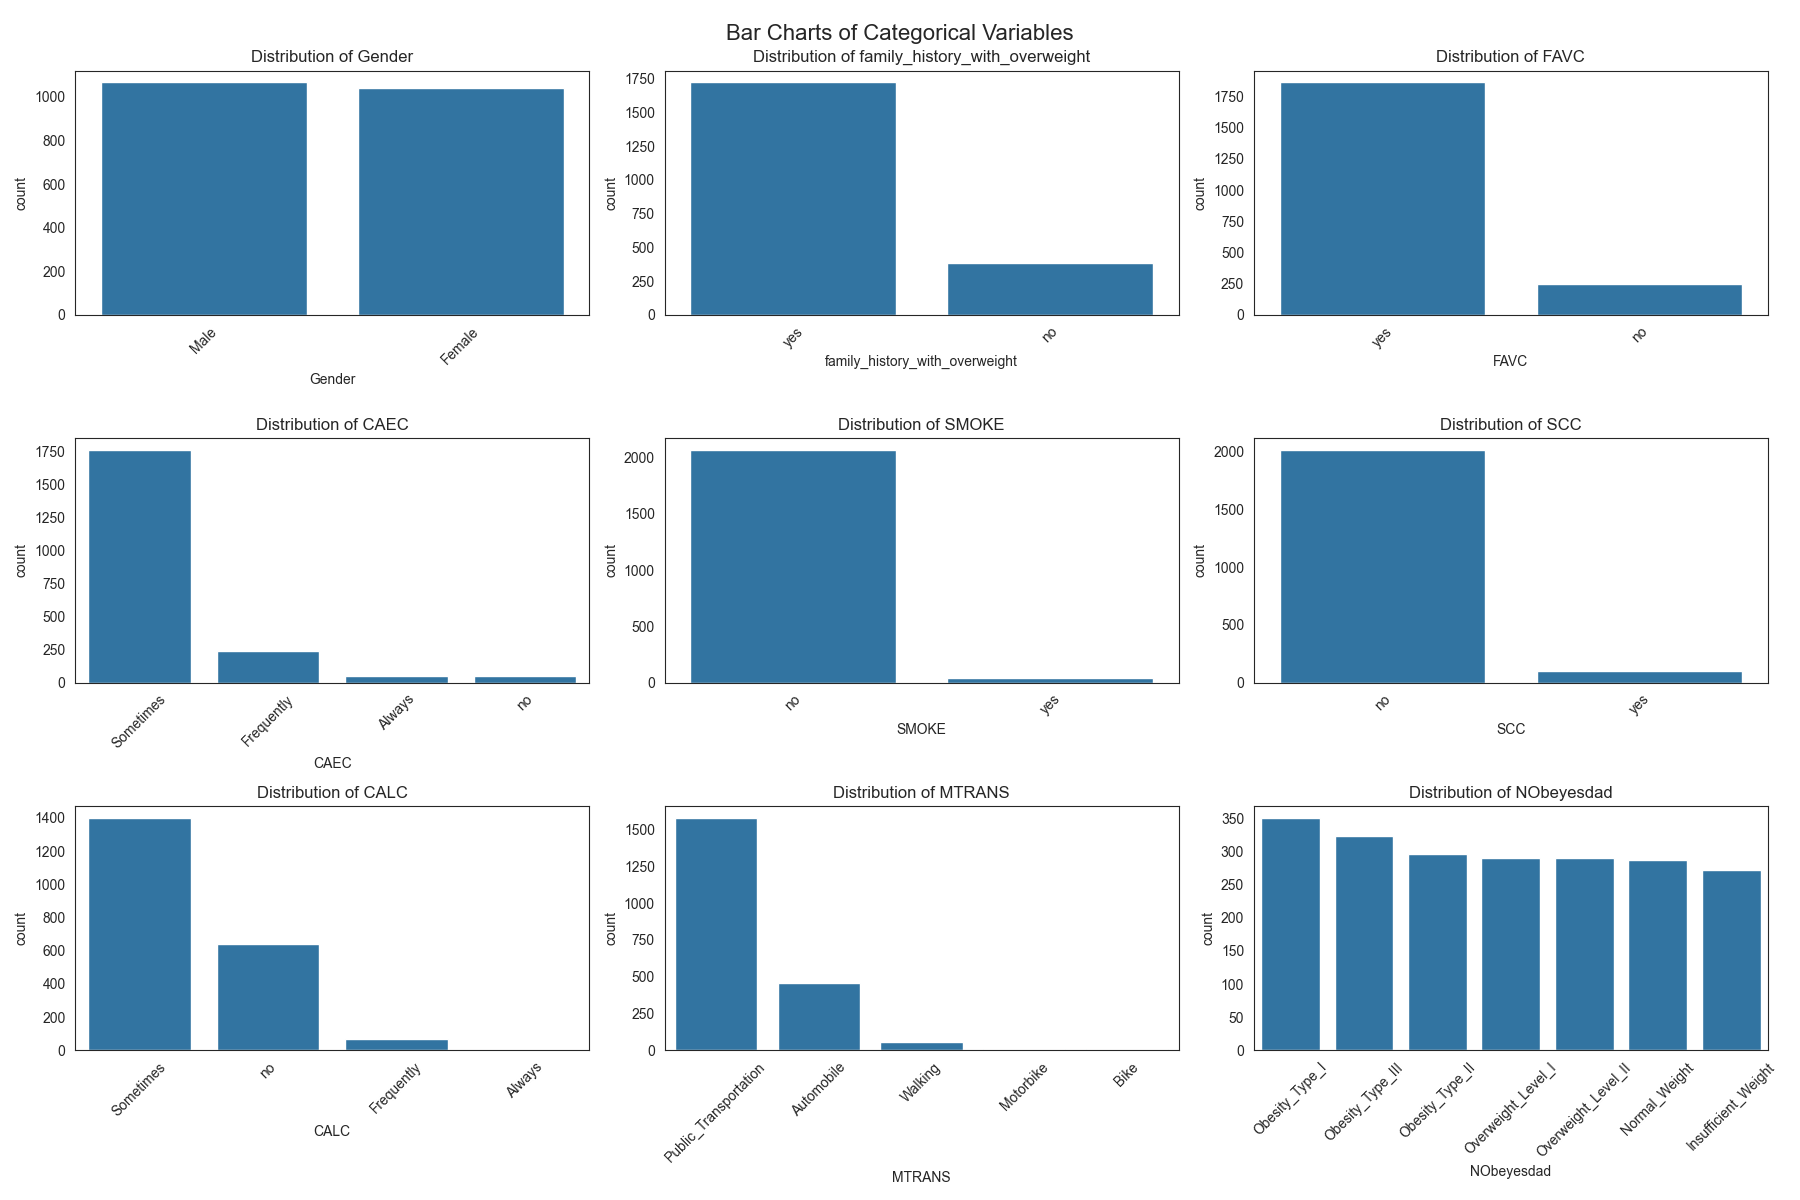
\includegraphics[width=0.8\textwidth]{BarCharts.png}
    \caption{Bar charts of categorical variables}
    \label{fig:bar_charts}
\end{figure}

After collapsing the response variable, I replotted the response variable, as seen below. While there is only a slight class imbalance, I still account for it later when I build the models.

\begin{figure}[H]
    \centering
    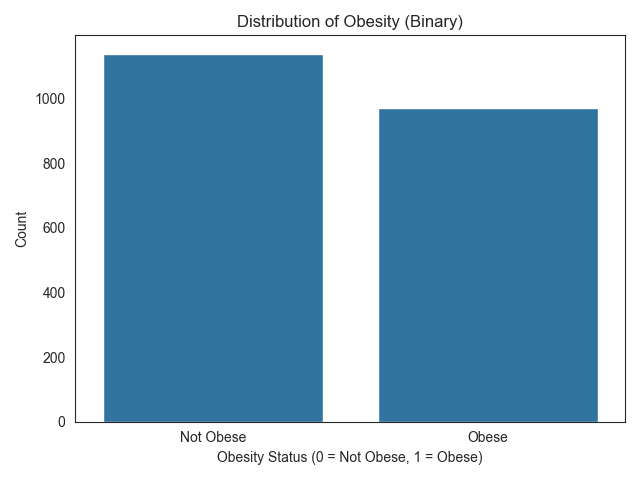
\includegraphics[width=0.6\textwidth]{ResponseDist.png}
    \caption{Distribution of the target variable}
    \label{fig:obese_binary_dist}
\end{figure}

I finally calculated and plotted a correlation matrix to observe the relationships between the variables in the dataset. While most variables showed insignificant correlations, the relationship between weight and the binary response variable, ObeseBinary, is, unsurprisingly, notable. For this reason, I ran two versions of this project with the same set of testing and training data, one with weight included in the model and one without, to observe the differences in performance and hyperparameter selection between the two variants.

\begin{figure}[H]
    \centering
    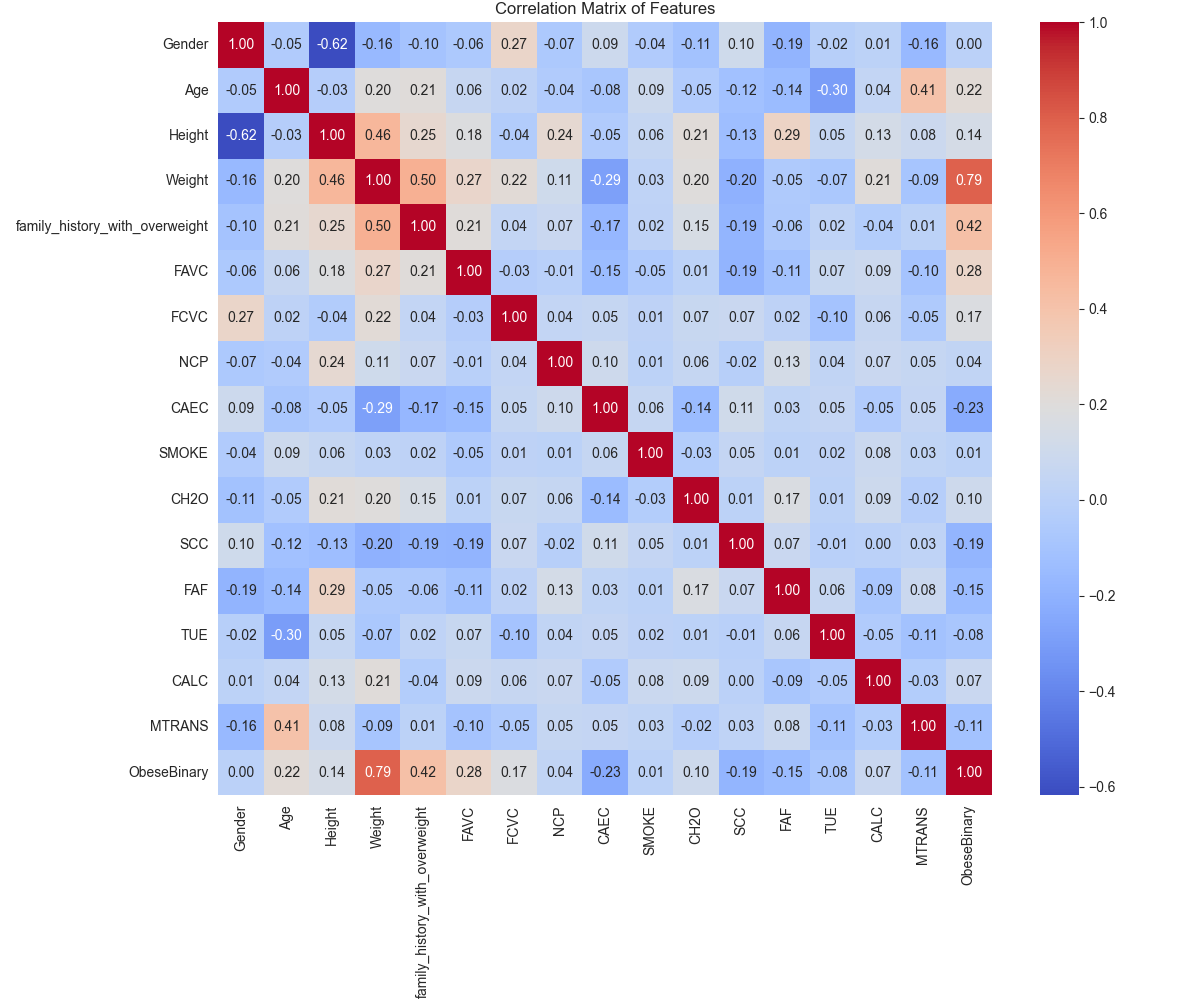
\includegraphics[width=0.85\textwidth]{CorrelationHeat.png}
    \caption{Correlation matrix for the obesity dataset}
    \label{fig:correlation_matrix}
\end{figure}

\section{Methods}
After separating my data into a stratified test/train split, I employed 8 methods on this dataset. For each method, I fit a baseline model, tuned the hyperparameters and cross-validated using Optuna, and finally evaluated the model on the held-out testing data. I finished the project by using permutation feature importance to compare different methods to determine which variables were most significant in each model. 

Each baseline model was fit using various packages from Python's sklearn library. Initially, no hyperparameters were specified; however, in models that learn by minimizing a loss function, such as Logistic Regression, SVM, Decision Trees, and Random Forests, I specified class weights to deal with the slight class imbalance observed in the target variable. The hyperparameters were tuned using Optuna, as mentioned above. Instead of grid search or random search, which can be either computationally demanding or unreliable, Optuna uses Bayesian optimization to efficiently explore the hyperparameter space. In this project, the objective was to maximize the balanced accuracy. Simultaneously, Optuna cross-validates each trial, making this method effective, computationally feasible, and statistically rigorous. After iterating through 50 trials, the best hyperparameters are then implemented into a final model, which evaluates the testing data, giving the final performance metrics and confusion matrices. Finally, I opted to use permutation feature importance to explore the importance of variables since it can be applied to all my models, making it ideal for comparison between methods.

The tuned hyperparameters and balanced accuracy for the tuned models and tables summarizing evaluation metrics for the trials with and without the weight variable are reported below. The confusion matrices for each variant of test data are also reported.\\

\textbf{k-NN:}
The optimal value of n-neighbor was 4, and the cross-validated balanced accuracy for the tuned k-NN model was 0.9510 for the variant with weight. In the variant without weight, the optimal value of n-neighbor was, again, 4, and the cross-validated accuracy was 0.9169.


\begin{table}[H]
\centering
\small
\begin{tabular}{lcccccc}
\toprule
\textbf{Class Weights} & \textbf{Accuracy} & \textbf{Balanced Acc.} & \textbf{Precision} & \textbf{Recall} & \textbf{F1 Score} & \textbf{ROC AUC} \\
\midrule
With Weight & 0.9504 & 0.9517 & 0.9265 & 0.9692 & 0.9474 & 0.9785 \\
Without Weight & 0.9220 & 0.9210 & 0.9219 & 0.9077 & 0.9147 & 0.9675 \\
\bottomrule
\end{tabular}
\caption{Evaluation metrics for k-NN with and without the weight variable}
\label{tab:knn_weights}
\end{table}

\begin{figure}[H]
\centering
\begin{minipage}{0.35\textwidth}
    \centering
    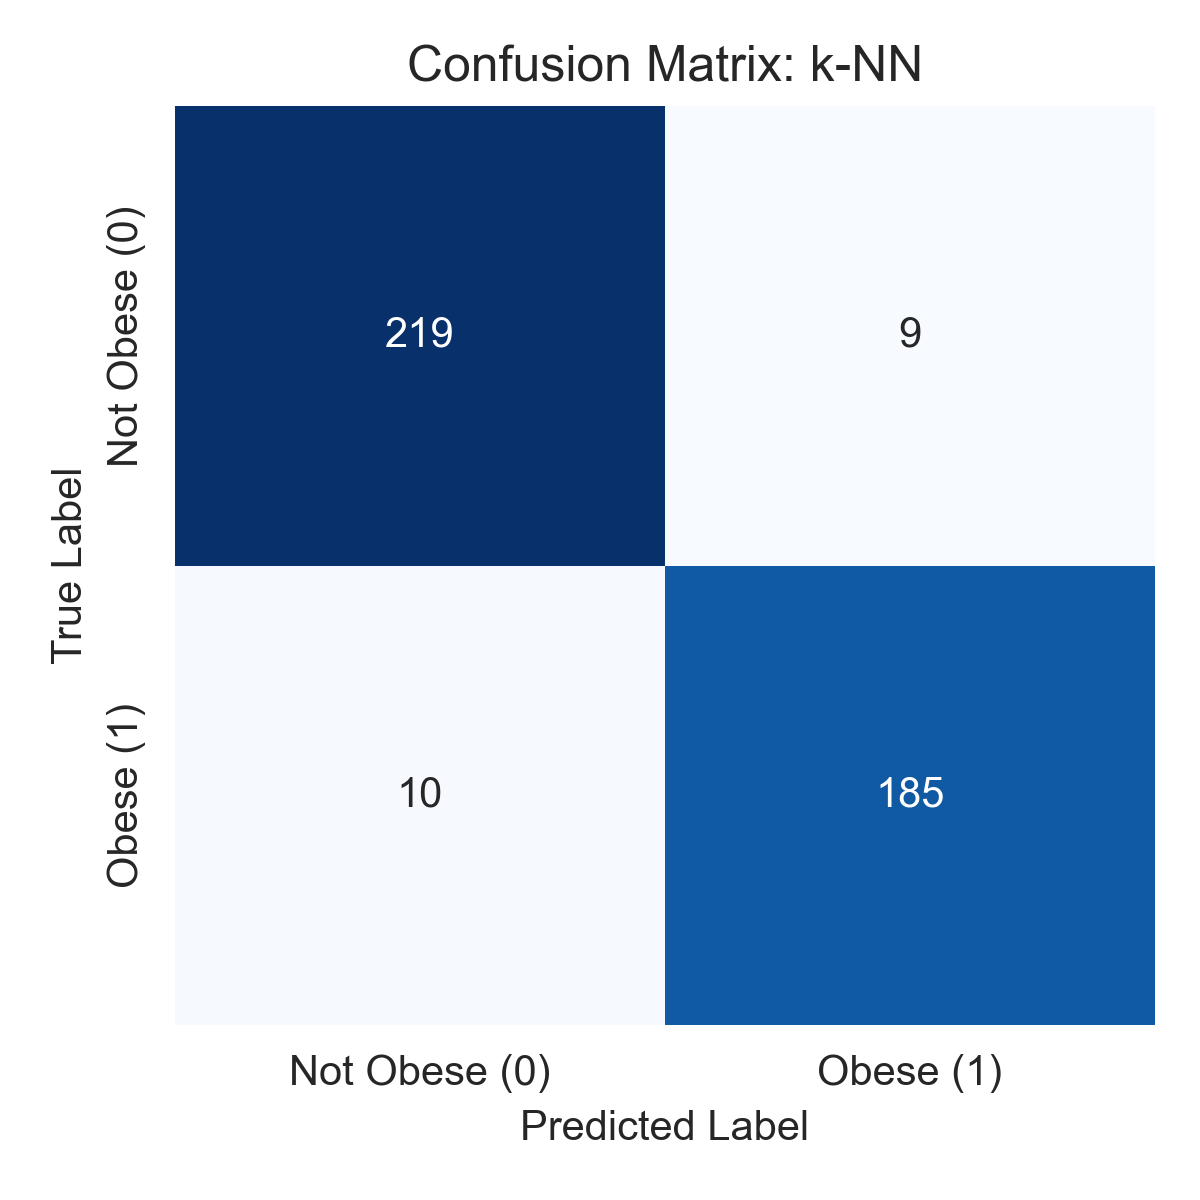
\includegraphics[width=\linewidth]{k-nn_confusion.png}
    \caption{k-NN Confusion Matrix (with weight)}
\end{minipage}
\hspace{0.04\textwidth}
\begin{minipage}{0.35\textwidth}
    \centering
    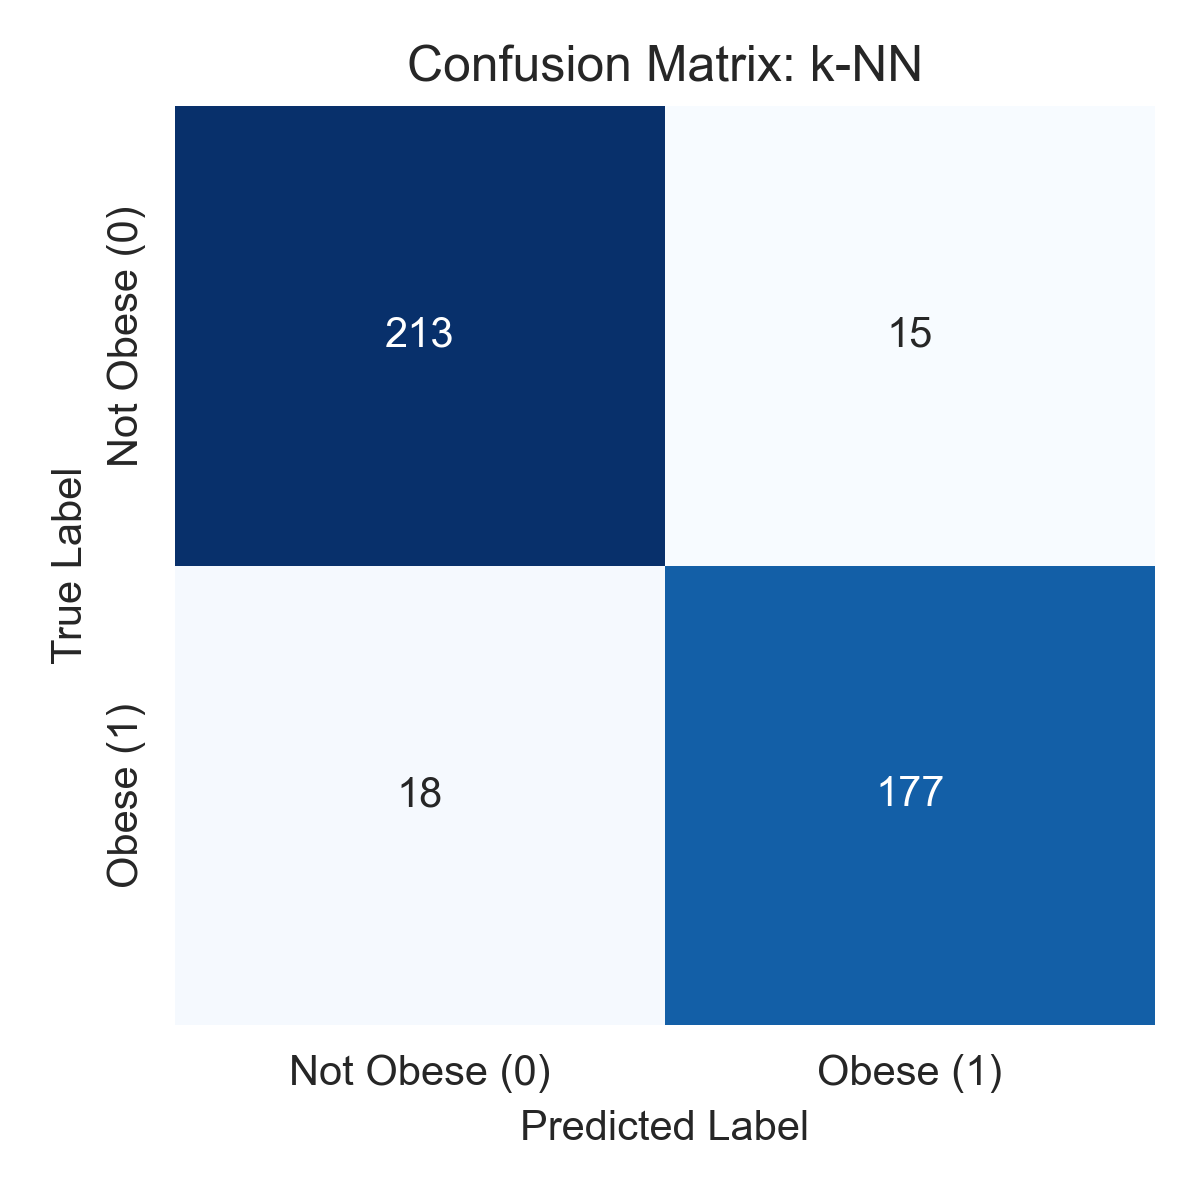
\includegraphics[width=\linewidth]{k-nn_confusion_withoutWeight.png}
    \caption{k-NN Confusion Matrix (without weight)}
\end{minipage}
\label{fig:k-nn_weight_comparison}
\end{figure}

In this model, the evaluation metrics seem fairly consistent across both variants of the analysis. While the model without weight did perform worse, that was unsurprising. Overall, the model seemed to classify the presence and lack of obesity equally. The number of nearest neighbors, n-neighbor, was the same for both analyses at 4. Interestingly, the cross-validated balanced accuracy was lower than the testing balanced accuracy for both variants of the analysis.

\textbf{LDA:}
Since LDA does not require hyperparameter tuning, it was evaluated directly using 5-fold cross-validation. The balanced accuracy achieved was 0.9698 in the variant with weight. In the variant without weight, the balanced accuracy was 0.7433.


\begin{table}[H]
\centering
\small
\begin{tabular}{lcccccc}
\toprule
\textbf{Class Weights} & \textbf{Accuracy} & \textbf{Balanced Acc.} & \textbf{Precision} & \textbf{Recall} & \textbf{F1 Score} & \textbf{ROC AUC} \\
\midrule
With Weight & 0.9764 & 0.9766 & 0.9695 & 0.9795 & 0.9745 & 0.9984 \\
Without Weight & 0.7589 & 0.7630 & 0.7067 & 0.8154 & 0.7571 & 0.8523 \\
\bottomrule
\end{tabular}
\caption{Evaluation metrics for LDA with and without the weight variable}
\label{tab:lda_weights}
\end{table}

\begin{figure}[H]
\centering
\begin{minipage}{0.35\textwidth}
    \centering
    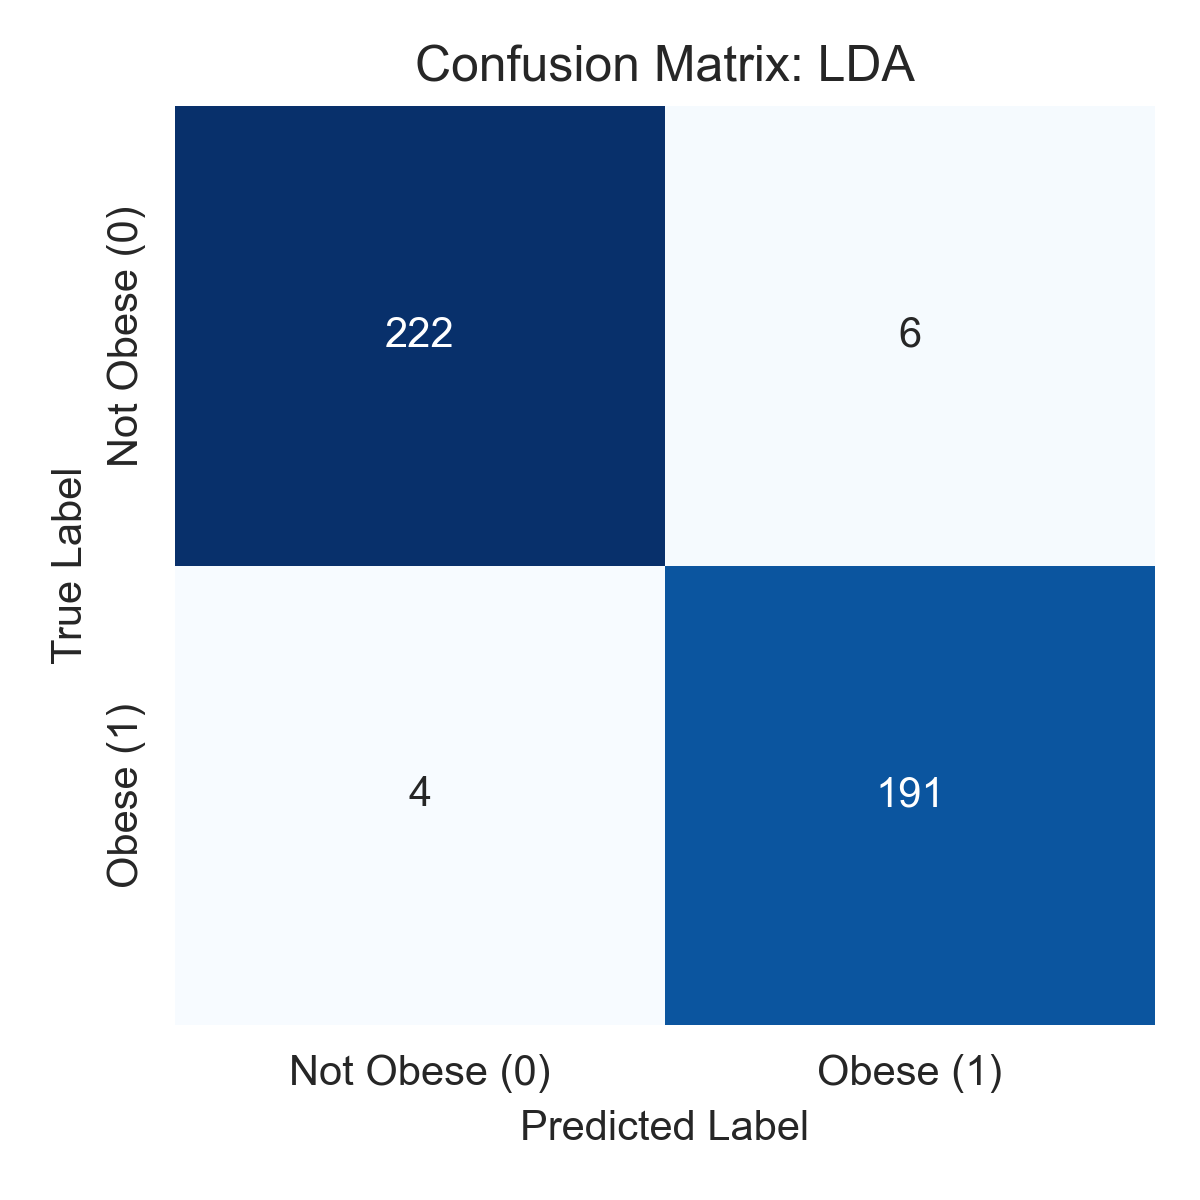
\includegraphics[width=\linewidth]{lda_confusion.png}
    \caption{LDA Confusion Matrix (with weight)}
\end{minipage}
\hspace{0.04\textwidth}
\begin{minipage}{0.35\textwidth}
    \centering
    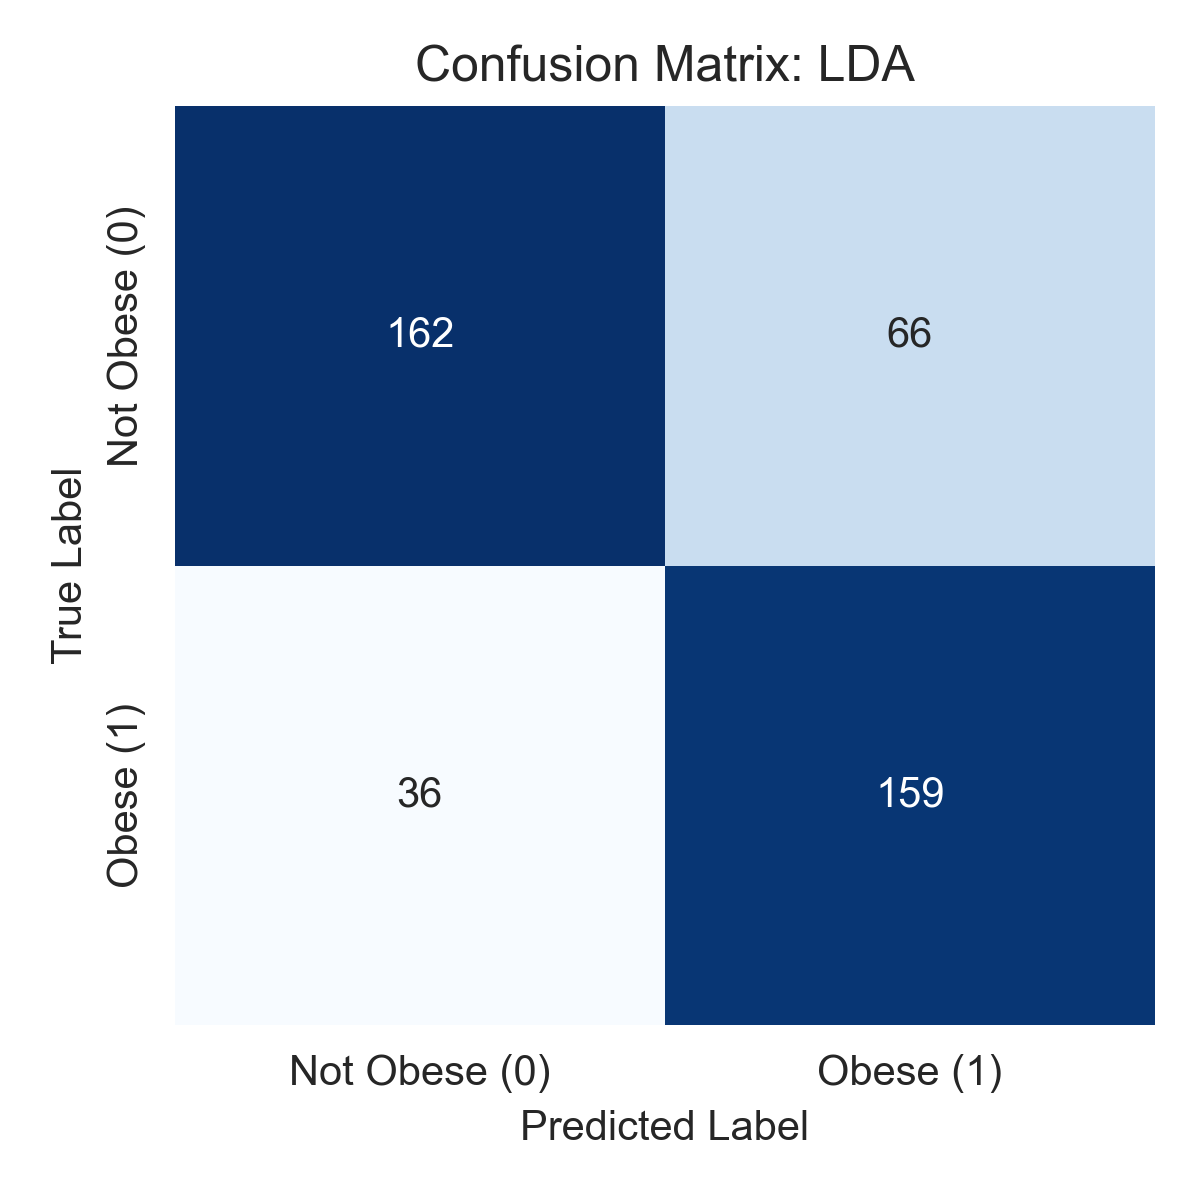
\includegraphics[width=\linewidth]{lda_confusion_withoutWeight.png}
    \caption{LDA Confusion Matrix (without weight)}
\end{minipage}
\label{fig:lda_weight_comparison}
\end{figure}

LDA performed significantly worse when weight was removed from the analysis, indicating weight was critical for this model to classify accurately. Regardless, the confusion matrices report fairly even misclassifications for both categories.

\textbf{QDA:}
Since QDA does not require hyperparameter tuning, it was evaluated directly using 5-fold cross-validation. The balanced accuracy achieved was 0.8696 in the variant with weight. In the variant without weight the balanced accuracy was 0.7880.


\begin{table}[H]
\centering
\small
\begin{tabular}{lcccccc}
\toprule
\textbf{Class Weights} & \textbf{Accuracy} & \textbf{Balanced Acc.} & \textbf{Precision} & \textbf{Recall} & \textbf{F1 Score} & \textbf{ROC AUC} \\
\midrule
With Weight & 0.8983 & 0.9024 & 0.8455 & 0.9538 & 0.8964 & 0.9756 \\
Without Weight & 0.8038 & 0.8143 & 0.7171 & 0.9487 & 0.8168 & 0.9353 \\
\bottomrule
\end{tabular}
\caption{Evaluation metrics for QDA with and without the weight variable}
\label{tab:qda_weights}
\end{table}

\begin{figure}[H]
\centering
\begin{minipage}{0.35\textwidth}
    \centering
    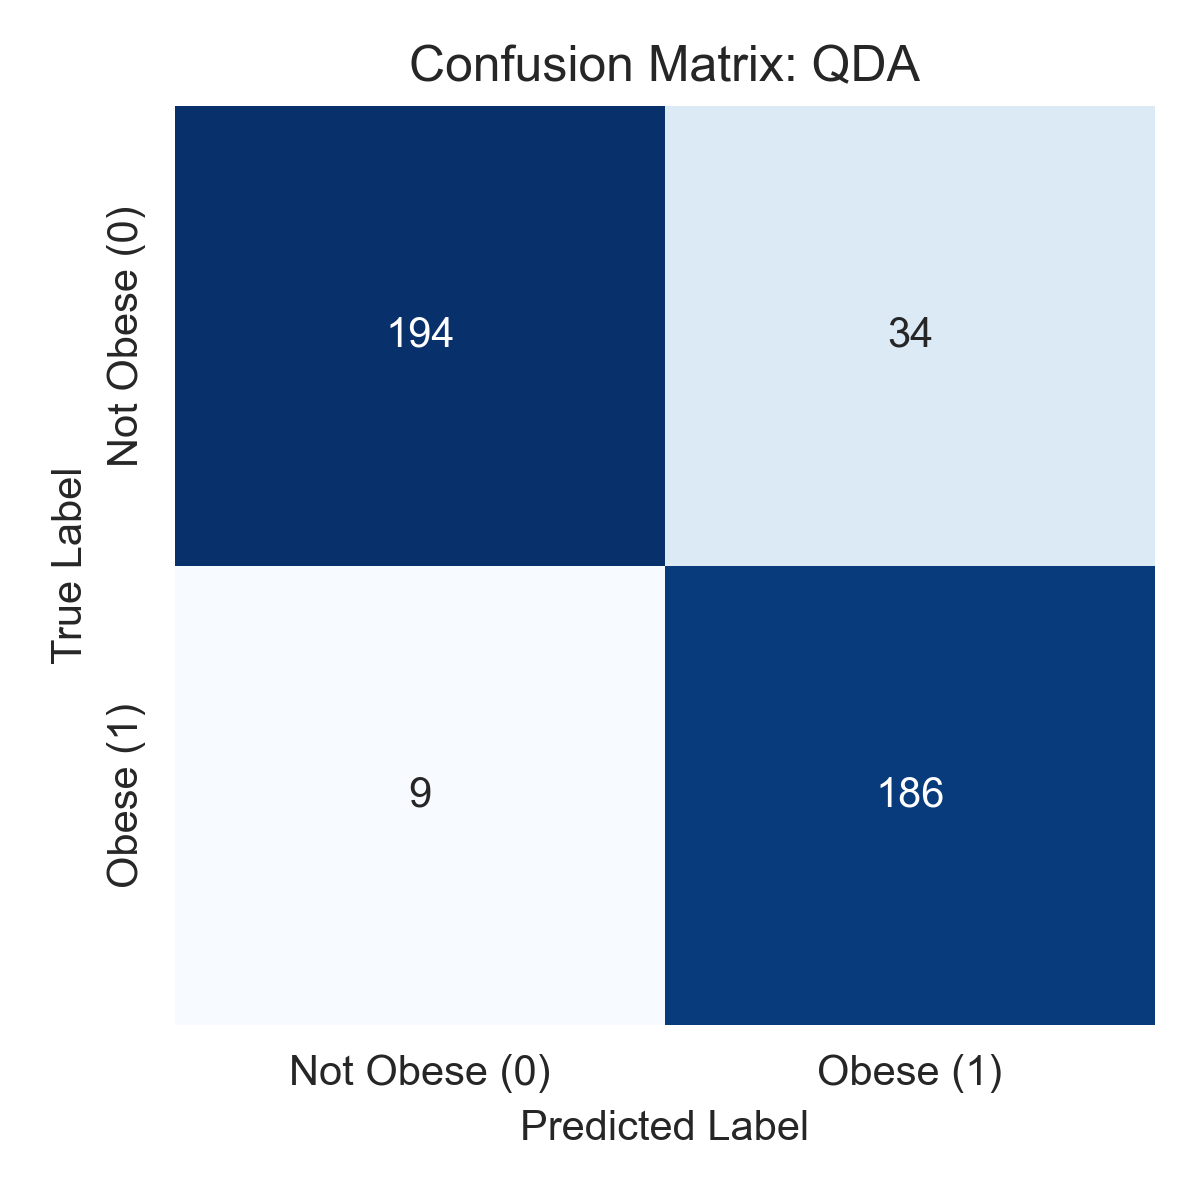
\includegraphics[width=\linewidth]{qda_confusion.png}
    \caption{QDA Confusion Matrix (with weight)}
\end{minipage}
\hspace{0.04\textwidth}
\begin{minipage}{0.35\textwidth}
    \centering
    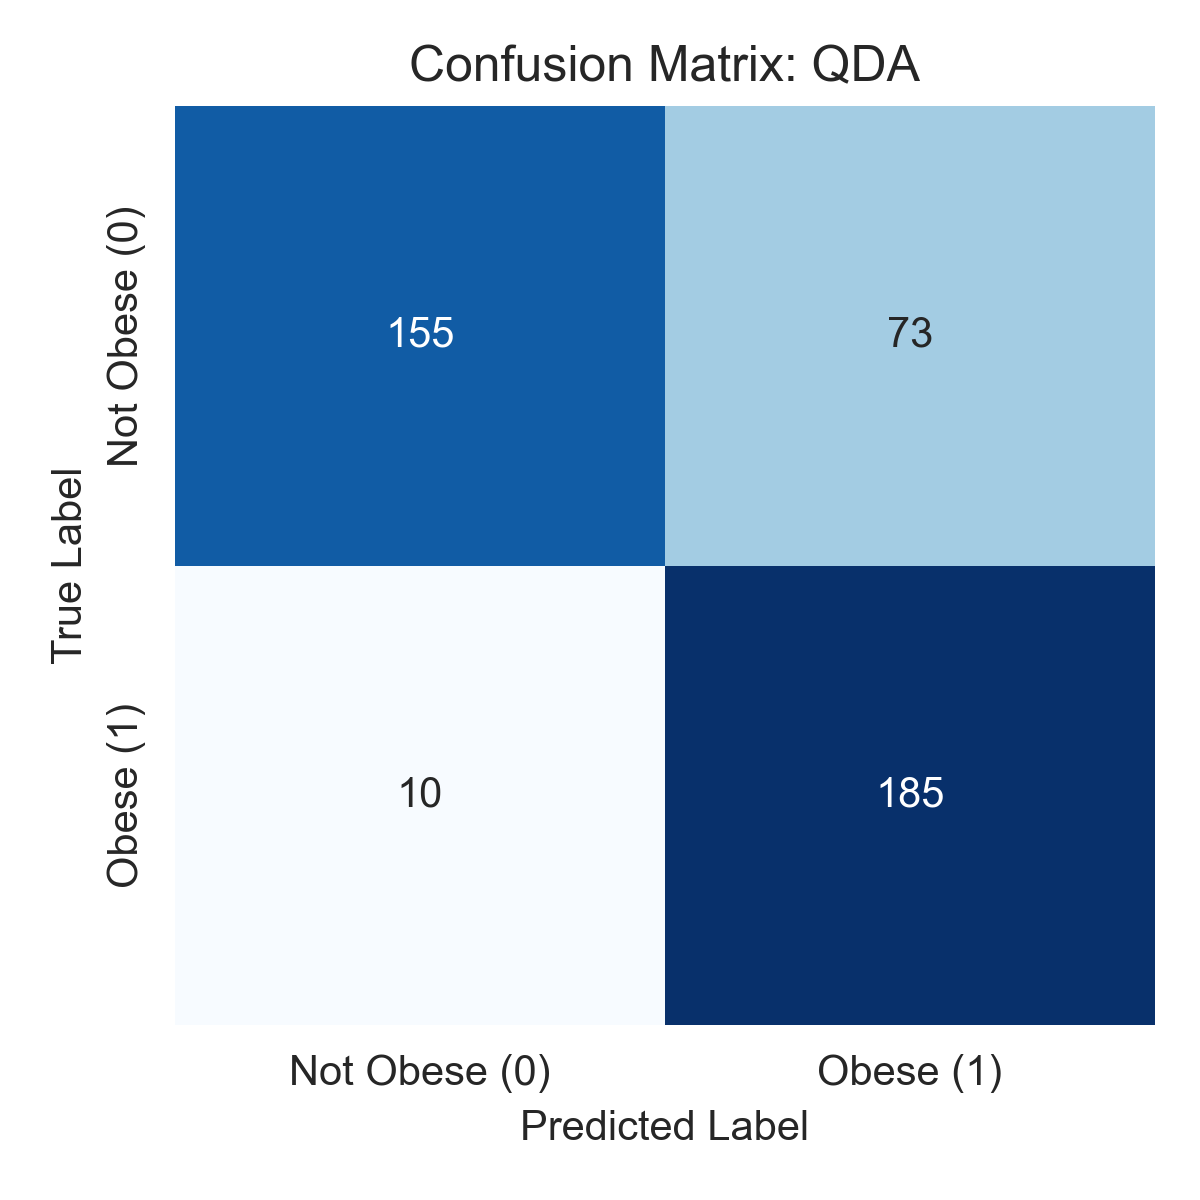
\includegraphics[width=\linewidth]{qda_confusion_withoutWeight.png}
    \caption{QDA Confusion Matrix (without weight)}
\end{minipage}
\label{fig:qda_weight_comparison}
\end{figure}

QDA also shows a significant drop in balanced accuracy from the model with weight to the model without weight, much like LDA. However, like k-NN, the cross-validated balanced accuracies are higher than the testing balanced accuracies. QDA also seems to misclassify those who are not obese at higher rates than other models, as is confirmed by the confusion matrices and low precision metric.

\textbf{Logistic Regression:}
The best parameters for Logistic Regression were penalty = $L_1$ and $C = 0.1277$. The cross-validated balanced accuracy was 0.9982 for the variant with weight. In the variant without weight, the best parameters were penalty = elasticnet and $c= 0.1250$. The optimal $L_1$ ratio was 0.3301 and the balanced accuracy was 0.7657.


\begin{table}[H]
\centering
\small
\begin{tabular}{lcccccc}
\toprule
\textbf{Class Weights} & \textbf{Accuracy} & \textbf{Balanced Acc.} & \textbf{Precision} & \textbf{Recall} & \textbf{F1 Score} & \textbf{ROC AUC} \\
\midrule
With Weight & 0.9976 & 0.9978 & 0.9949 & 1.0000 & 0.9974 & 1.0000 \\
Without Weight & 0.7849 & 0.7908 & 0.7222 & 0.8667 & 0.7879 & 0.8614 \\
\bottomrule
\end{tabular}
\caption{Evaluation metrics for Logistic Regression with and without the weight variable}
\label{tab:logreg_weights}
\end{table}

\begin{figure}[H]
\centering
\begin{minipage}{0.35\textwidth}
    \centering
    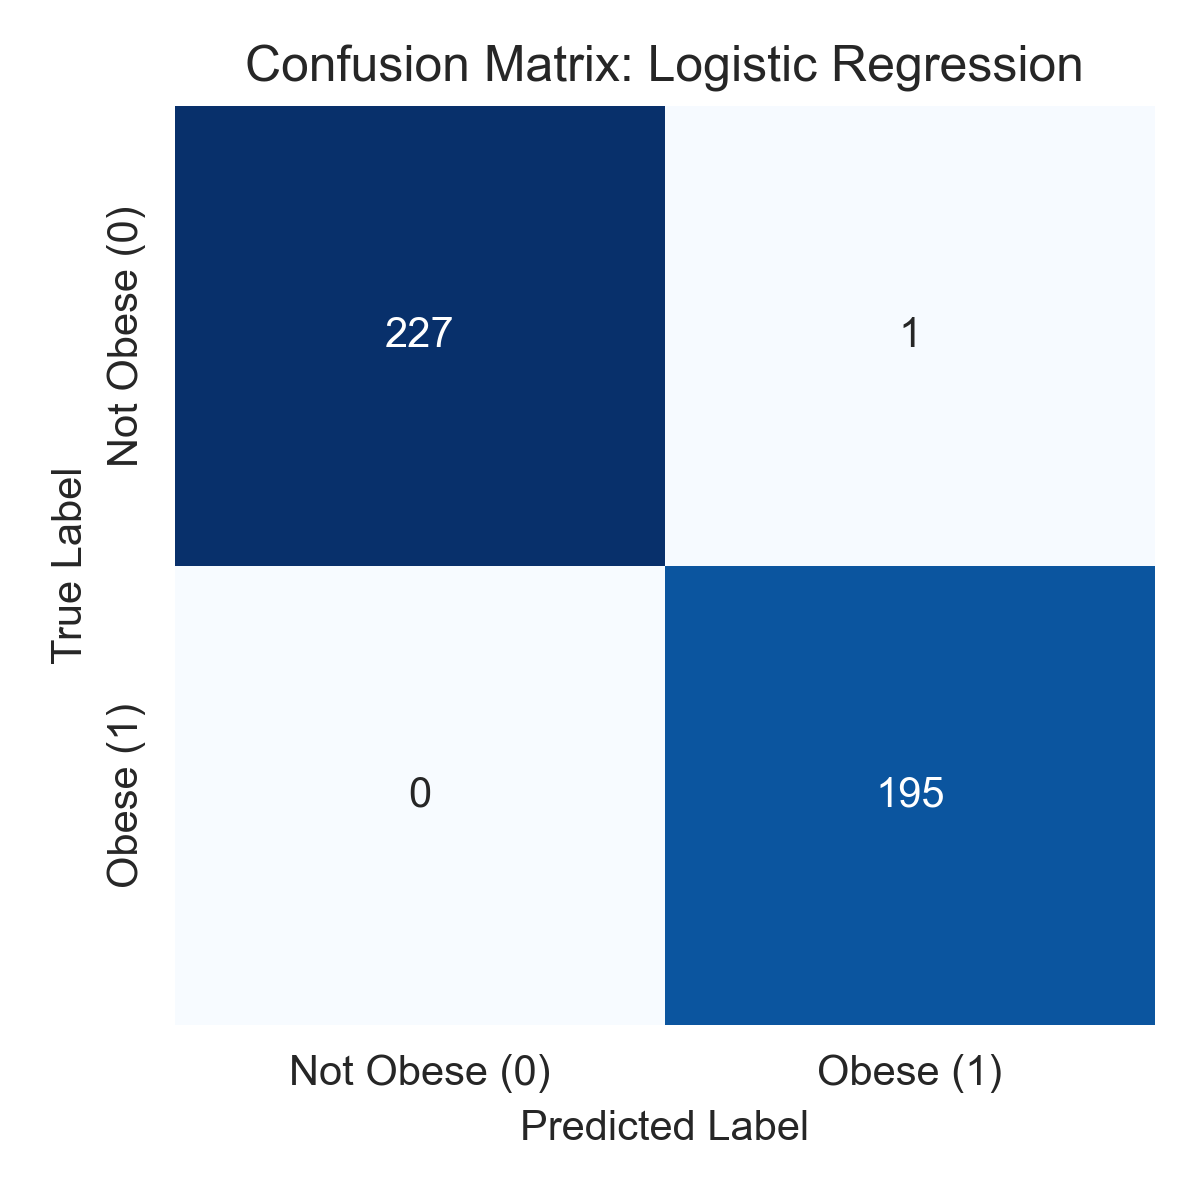
\includegraphics[width=\linewidth]{logistic_regression_confusion.png}
    \caption{Logistic Regression Confusion Matrix (with weight)}
\end{minipage}
\hspace{0.04\textwidth}
\begin{minipage}{0.35\textwidth}
    \centering
    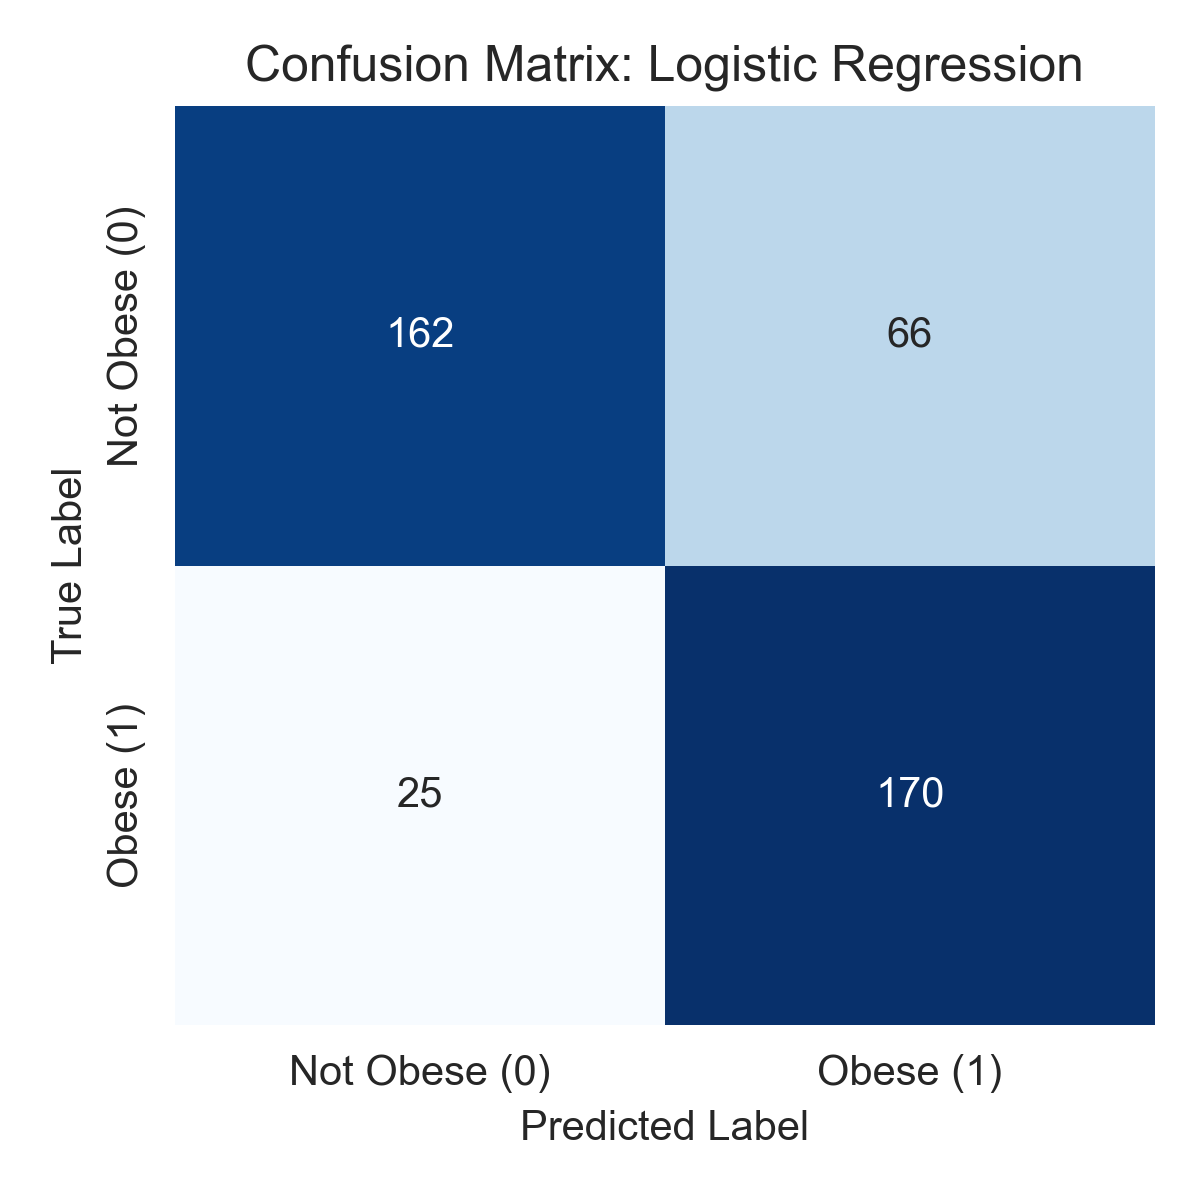
\includegraphics[width=\linewidth]{logistic_regression_confusion_withoutWeight.png}
    \caption{Logistic Regression Confusion Matrix (without weight)}
\end{minipage}
\label{fig:logreg_weight_comparison}
\end{figure}

For the logistic regression models, Optuna found different regularization methods were best when the analysis did and did not contain the weight variable. For the model with weight, it found $L_1$ regularization, or LASSO regression, was best for the data. Without weight, it found elastic net regularization, a combination of $L_1$ and $L_2$ penalties, was better. This model saw significant drops in balanced accuracy from one variant to the other. Surprisingly, the model with weight had perfect recall, and only misclassified one observation. In the model without weight, it seems to have lower precision, which is confirmed by looking at the misclassification distribution in the confusion matrix. 

\textbf{Decision Tree:}
The optimal hyperparameters for the Decision Tree model were max\_depth = 7, min\_samples\_split = 3, and min\_samples\_leaf = 7 and the cross-validated balanced accuracy was 0.9911 for the variant with weight. In the variant without weight, the best hyperparameters were max\_depth = 17, min\_samples\_split = 8, and min\_samples\_leaf = 8. The balanced accuracy was 0.8877.

\begin{table}[H]
\centering
\small
\begin{tabular}{lcccccc}
\toprule
\textbf{Class Weights} & \textbf{Accuracy} & \textbf{Balanced Acc.} & \textbf{Precision} & \textbf{Recall} & \textbf{F1 Score} & \textbf{ROC AUC} \\
\midrule
With Weight & 0.9764 & 0.9773 & 0.9602 & 0.9897 & 0.9747 & 0.9900 \\
Without Weight & 0.9173 & 0.9184 & 0.8922 & 0.9333 & 0.9123 & 0.9474 \\
\bottomrule
\end{tabular}
\caption{Evaluation metrics for Decision Tree with and without the weight variable}
\label{tab:dtree_weights}
\end{table}

\begin{figure}[H]
\centering
\begin{minipage}{0.35\textwidth}
    \centering
    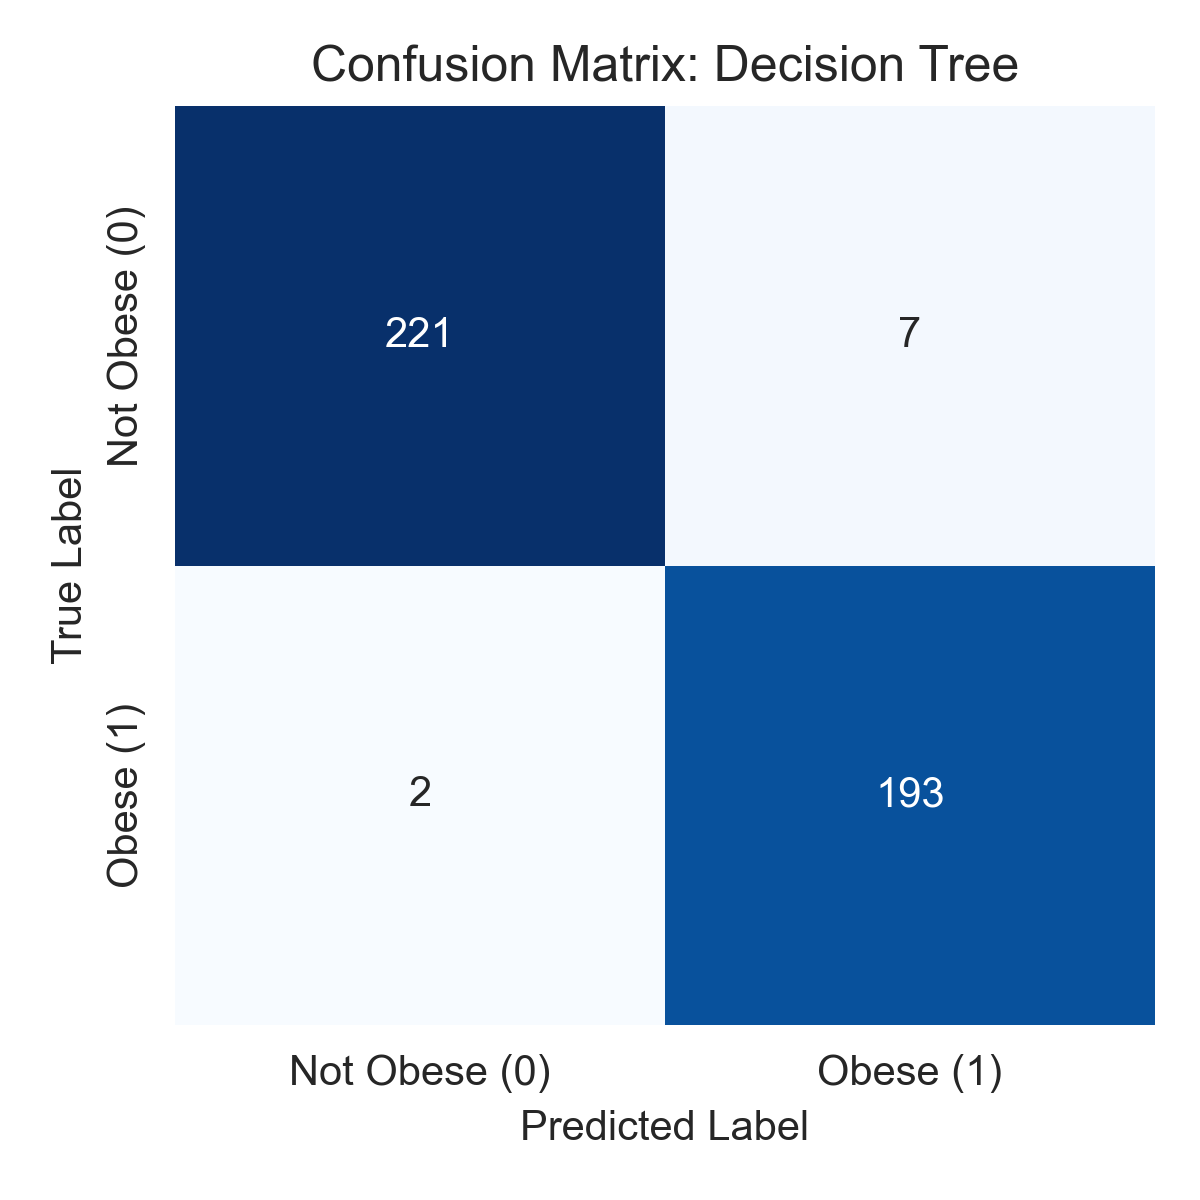
\includegraphics[width=\linewidth]{decision_tree_confusion.png}
    \caption{Decision Tree Confusion Matrix (with weight)}
\end{minipage}
\hspace{0.04\textwidth}
\begin{minipage}{0.35\textwidth}
    \centering
    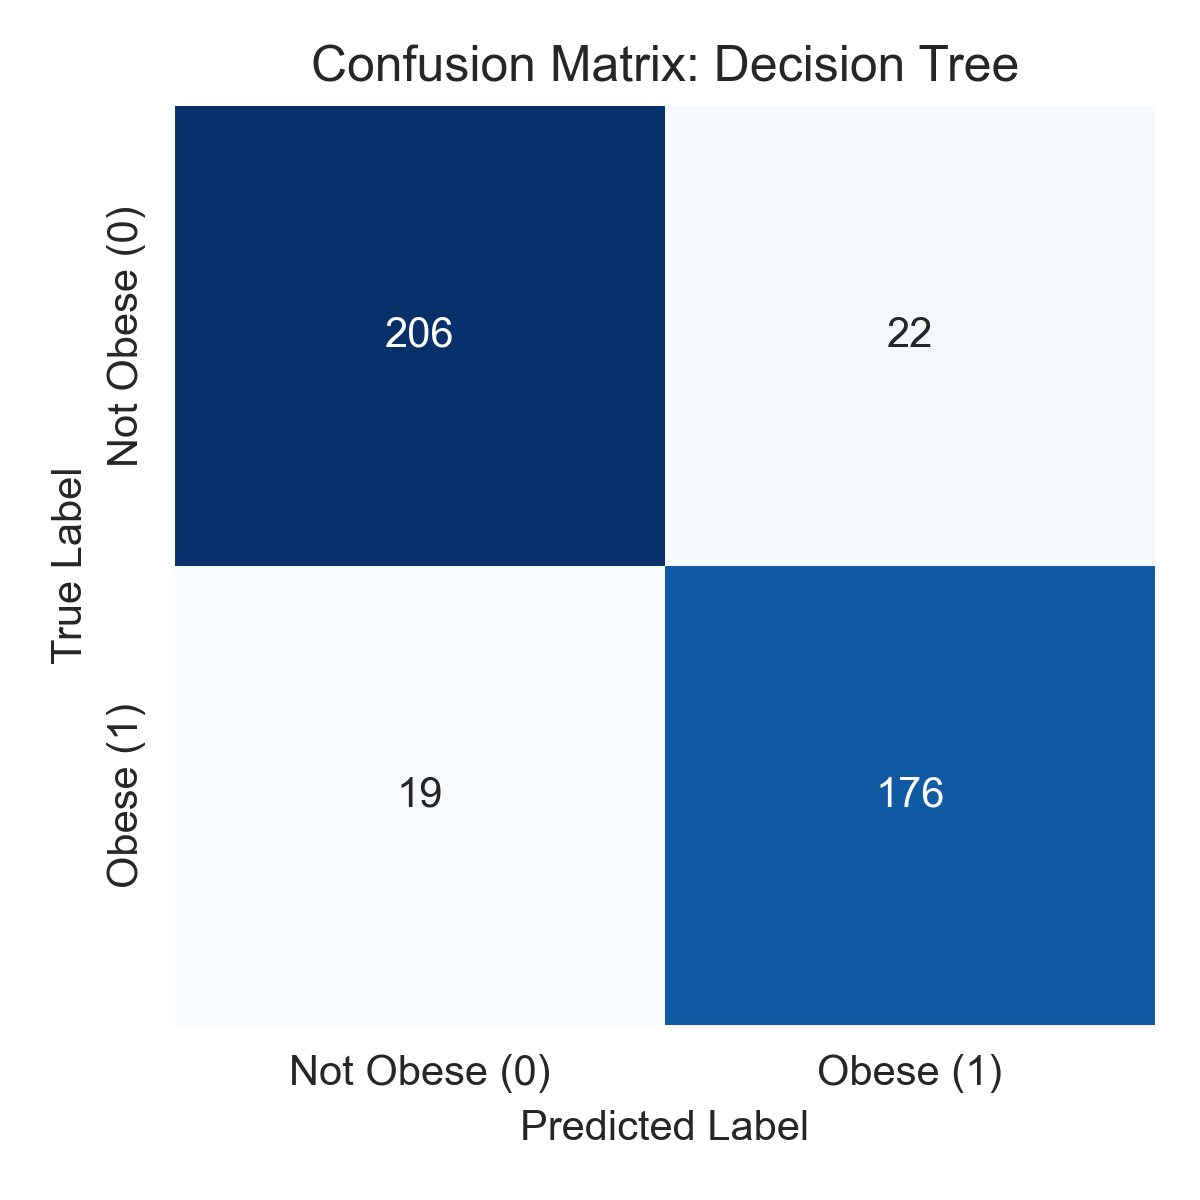
\includegraphics[width=\linewidth]{decision_tree_confusion_withoutWeight.png}
    \caption{Decision Tree Confusion Matrix (without weight)}
\end{minipage}
\label{fig:decision_weight_comparison}
\end{figure}

The decision tree model in both variants of the analysis were well balanced. It doesn't seem to misclassify one class much more than the other. While the balanced accuracy drops when weight is removed from the analysis, the balanced accuracies are higher than the cross-validated balanced accuracies. The maximum depth of the tree also varied widely with and without weight in the model. With weight, it had a maximum depth of 7, which jumped to 17 when weight was removed from the model.

\textbf{Random Forest:}
The best configuration for the Random Forest was n\_estimators = 146, max\_depth = 14, min\_samples\_split = 2, and min\_samples\_leaf = 1 and it achieved a balanced accuracy of 0.9928 in the variant with weight. For the variant without weight, the best hyperparameters were n\_estimators = 159, max\_depth = 16, min\_samples\_split = 3, and min\_samples\_leaf = 1. The balanced accuracy was 0.9432.
 
\begin{table}[H]
\centering
\small
\begin{tabular}{lcccccc}
\toprule
\textbf{Class Weights} & \textbf{Accuracy} & \textbf{Balanced Acc.} & \textbf{Precision} & \textbf{Recall} & \textbf{F1 Score} & \textbf{ROC AUC} \\
\midrule
With Weight & 0.9929 & 0.9927 & 0.9948 & 0.9897 & 0.9923 & 0.9999 \\
Without Weight & 0.9669 & 0.9660 & 0.9738 & 0.9538 & 0.9637 & 0.9876 \\
\bottomrule
\end{tabular}
\caption{Evaluation metrics for Random Forest with and without the weight variable}
\label{tab:rf_weights}
\end{table}

\begin{figure}[H]
\centering
\begin{minipage}{0.35\textwidth}
    \centering
    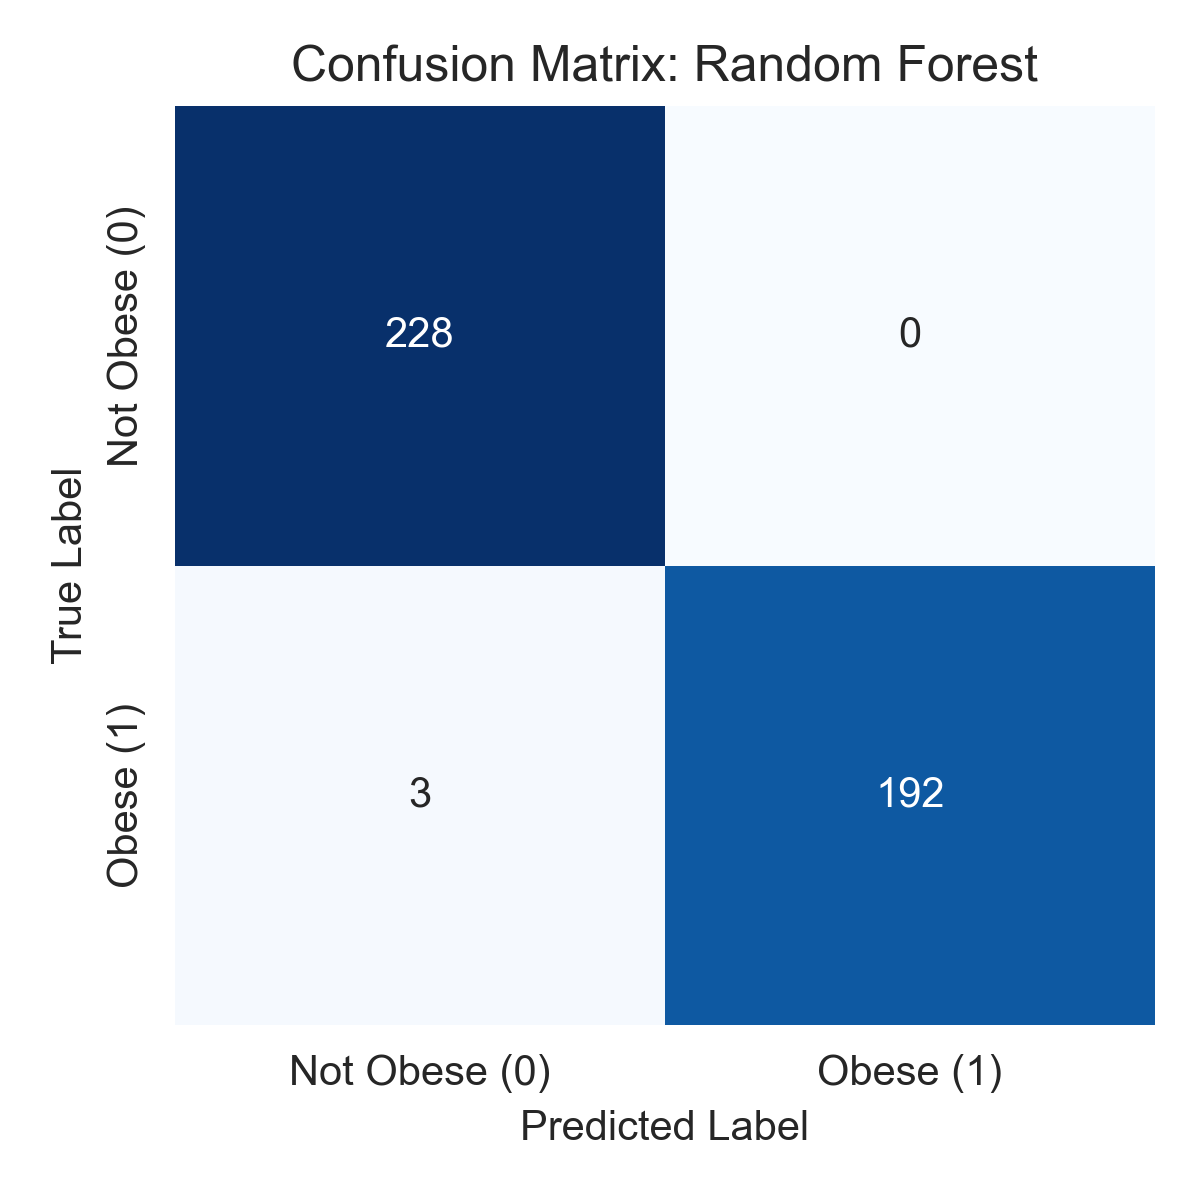
\includegraphics[width=\linewidth]{random_forest_confusion.png}
    \caption{Random Forest Confusion Matrix (with weight)}
\end{minipage}
\hspace{0.04\textwidth}
\begin{minipage}{0.35\textwidth}
    \centering
    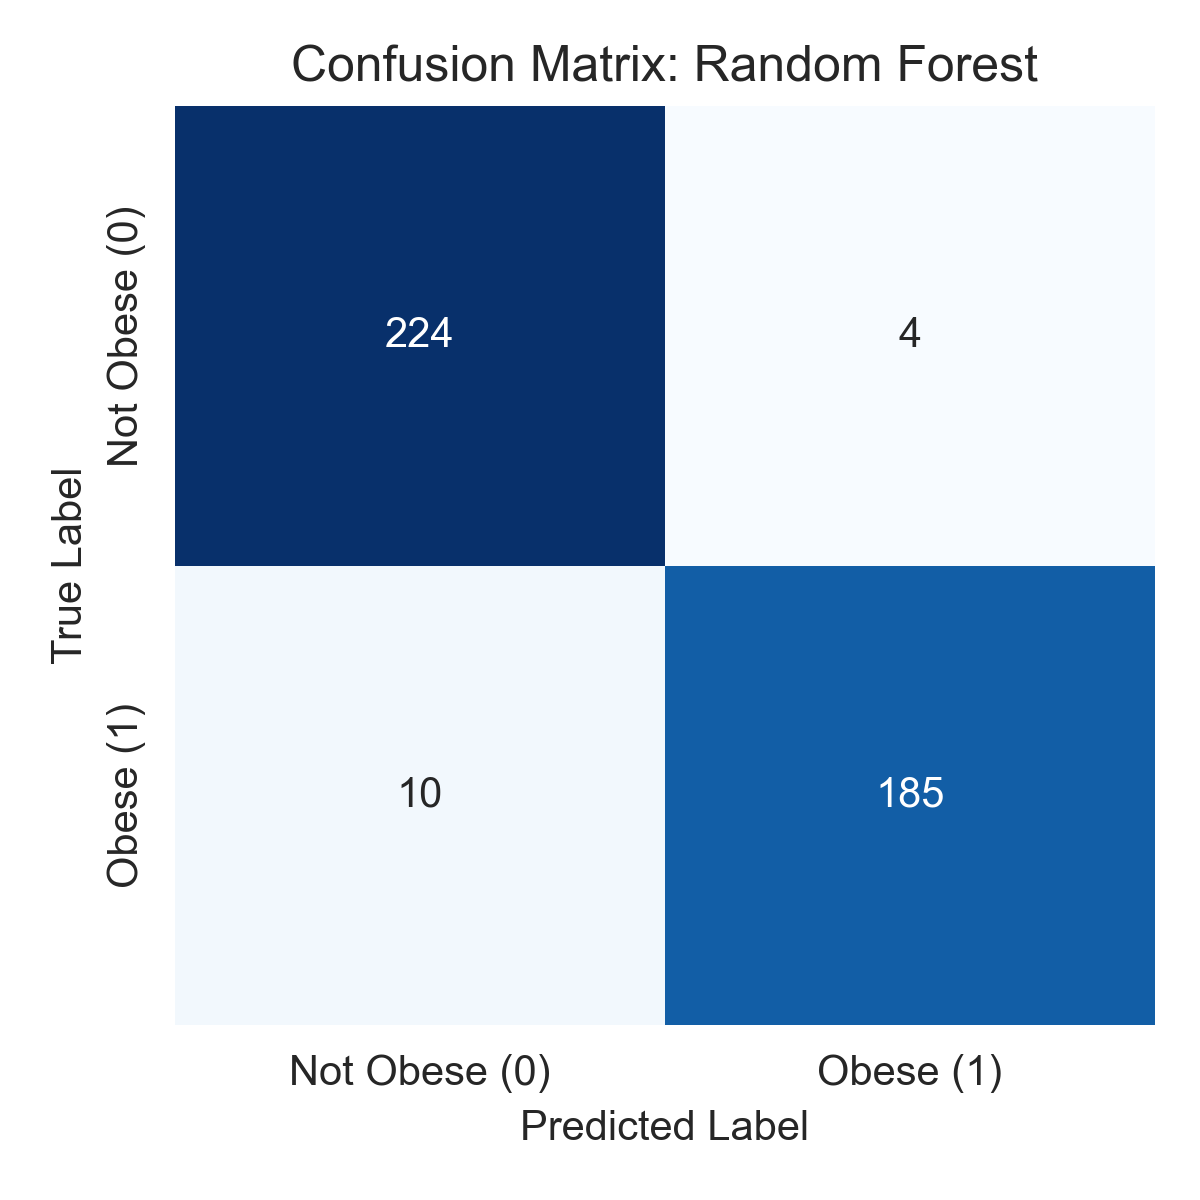
\includegraphics[width=\linewidth]{random_forest_confusion_withoutWeight.png}
    \caption{Random Forest Confusion Matrix (without weight)}
\end{minipage}
\label{fig:Random_Forest_weight_comparison}
\end{figure}

The results of the random forest model were quite comparable between the analysis with and without weight. There are slight variations the the optimal model hyperparameters, and balanced accuracy did drop slightly when weight was removed, but it remained fairly consistent from one to the other.

\textbf{Gradient Boosting:}
The tuned Gradient Boosting model used n\_estimators = 64, learning\_rate = 0.2058, max\_depth = 4, and subsample = 0.6816 and the balanced accuracy from cross-validation was 0.9953 for the variant with weight. In the variant without weight, the tuned model used n\_estimators = 125, learning\_rate = 0.1198, max\_depth = 10, and subsample = 0.7758. The balanced accuracy was 0.9513. 

\begin{table}[H]
\centering
\small
\begin{tabular}{lcccccc}
\toprule
\textbf{Class Weights} & \textbf{Accuracy} & \textbf{Balanced Acc.} & \textbf{Precision} & \textbf{Recall} & \textbf{F1 Score} & \textbf{ROC AUC} \\
\midrule
With Weight & 0.9976 & 0.9974 & 1.0000 & 0.9949 & 0.9974 & 1.0000 \\
Without Weight & 0.9764 & 0.9755 & 0.9843 & 0.9641 & 0.9741 & 0.9910 \\
\bottomrule
\end{tabular}
\caption{Evaluation metrics for Gradient Boosting with and without the weight variable}
\label{tab:gb_weights}
\end{table}

\begin{figure}[H]
\centering
\begin{minipage}{0.35\textwidth}
    \centering
    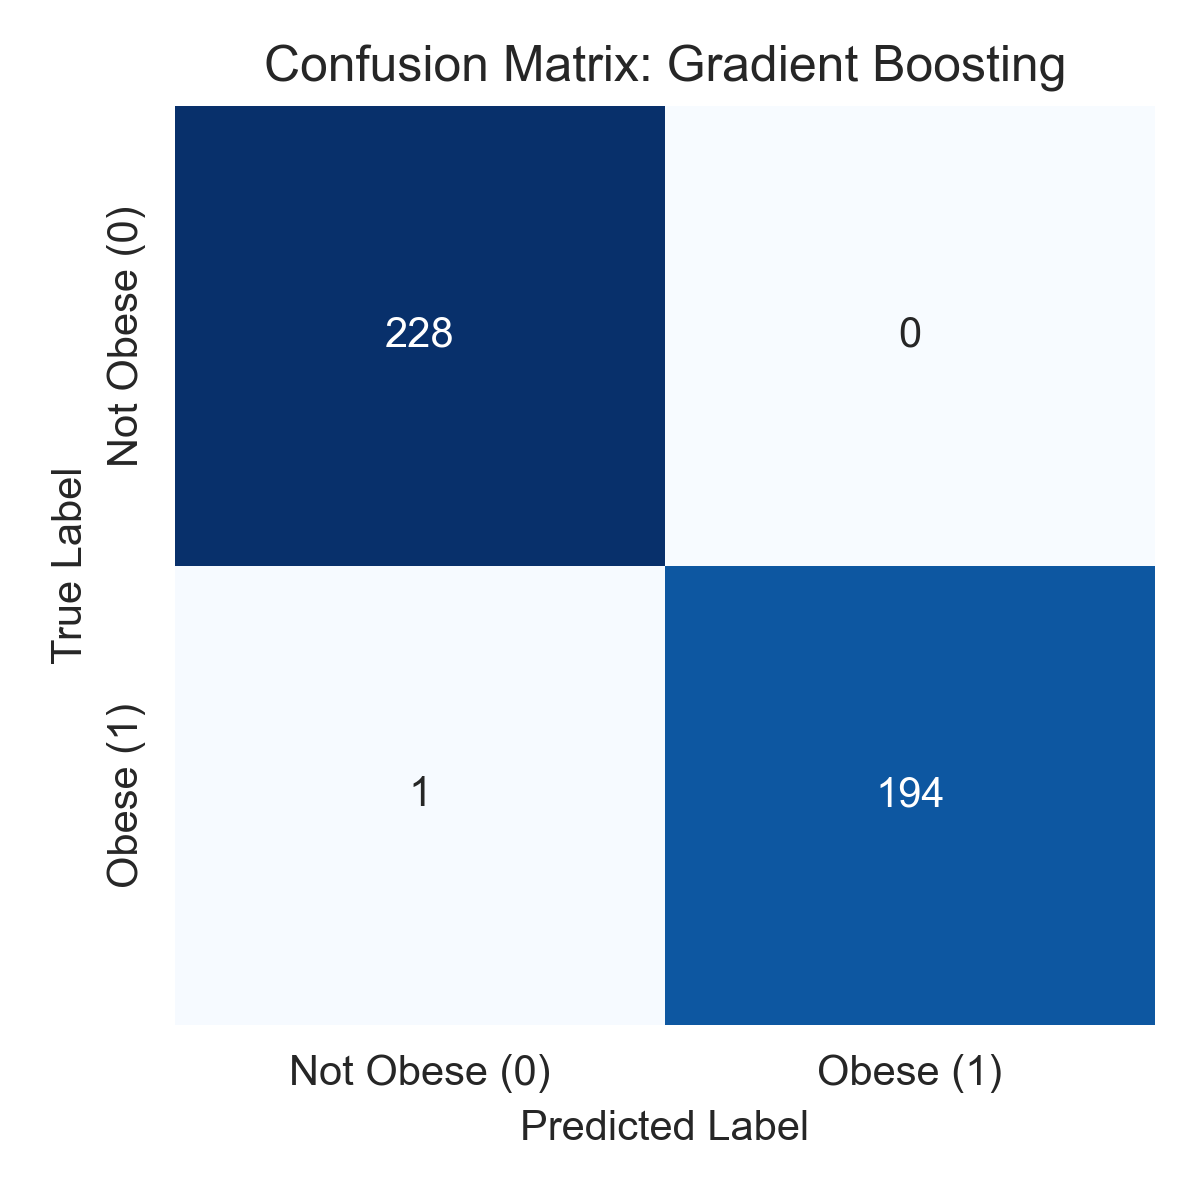
\includegraphics[width=\linewidth]{gradient_boosting_confusion.png}
    \caption{Gradient Boosting Confusion Matrix (with weight)}
\end{minipage}
\hspace{0.04\textwidth}
\begin{minipage}{0.35\textwidth}
    \centering
    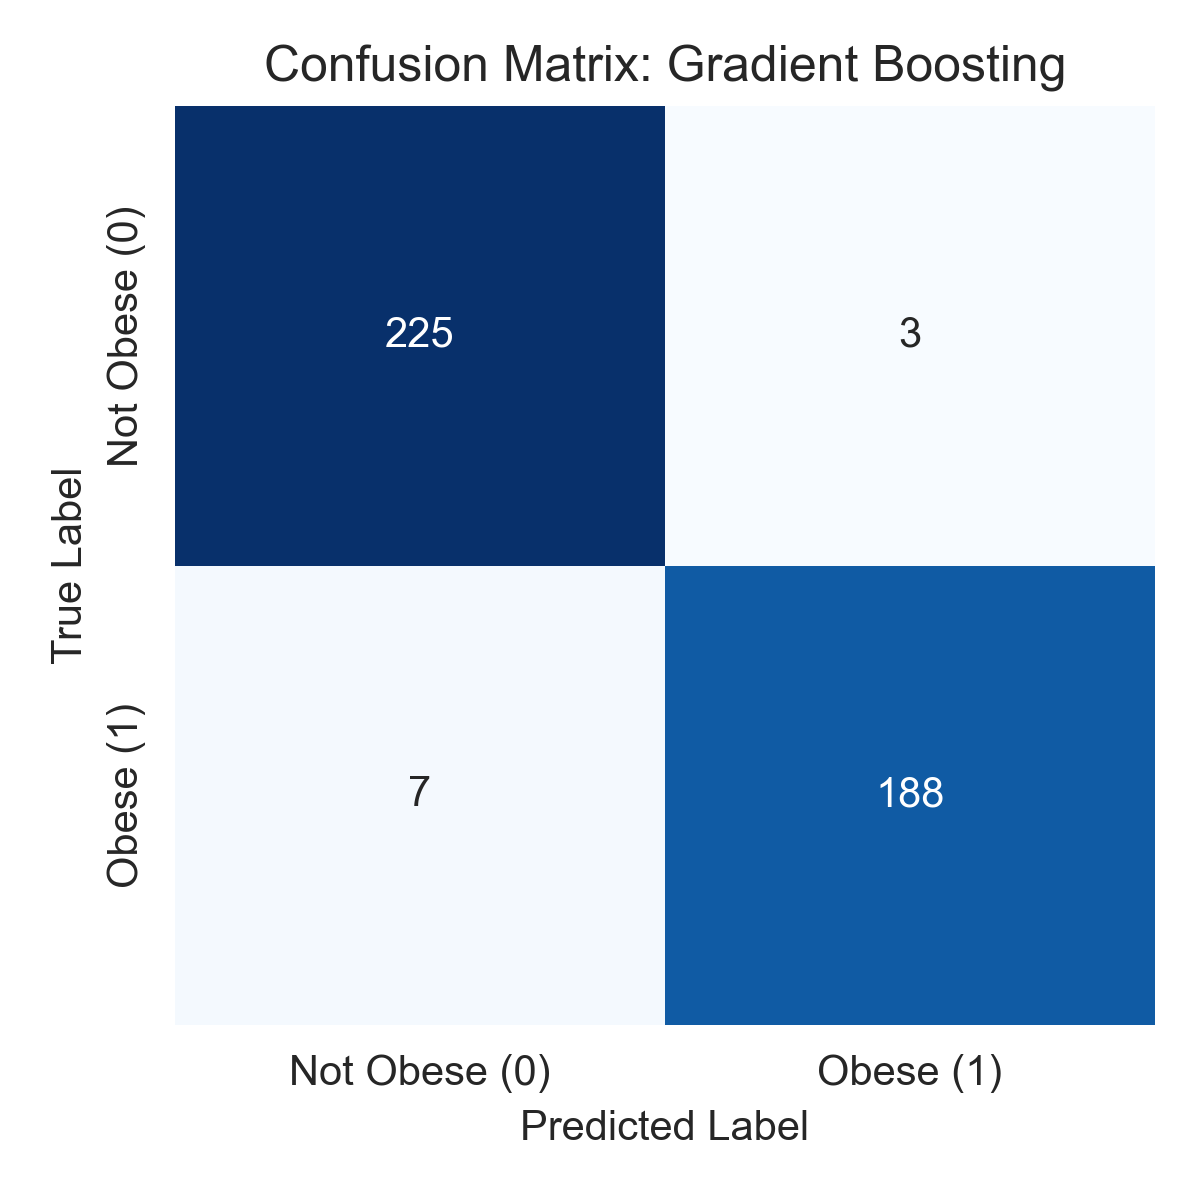
\includegraphics[width=\linewidth]{gradient_boosting_confusion_withoutWeight.png}
    \caption{Gradient Boosting Confusion Matrix (without weight)}
\end{minipage}
\label{fig:gb_weight_comparison}
\end{figure}

This model boasts high balanced accuracies, unsurprising for gradient boosting, which is known for strong accuracy rates. There was a negligible drop in balanced accuracy when weight was removed from the analysis. Like logistic regression, when weight was included, there was only 1 misclassification. The model hyperparameters do vary widely with and without weight, but that is to be expected, considering gradient boosting is known for its granularity.  

\textbf{SVM:}
The best hyperparameters for SVM were $C = 9.4319$ and $\gamma = 0.0079$, and the balanced accuracy from cross-validation was 0.9921 for the variant with weight. In the variant without weight, the best hyperparameters were $C = 3.3828$ and $\gamma = 0.0963$. The balanced accuracy was 0.9172.

\begin{table}[H]
\centering
\small
\begin{tabular}{lcccccc}
\toprule
\textbf{Class Weights} & \textbf{Accuracy} & \textbf{Balanced Acc.} & \textbf{Precision} & \textbf{Recall} & \textbf{F1 Score} & \textbf{ROC AUC} \\
\midrule
With Weight & 0.9905 & 0.9909 & 0.9848 & 0.9949 & 0.9898 & 0.9998 \\
Without Weight & 0.9338 & 0.9334 & 0.9282 & 0.9282 & 0.9282 & 0.9763 \\
\bottomrule
\end{tabular}
\caption{Evaluation metrics for SVM with and without the weight variable}
\label{tab:svm_weights}
\end{table}

\begin{figure}[H]
\centering
\begin{minipage}{0.35\textwidth}
    \centering
    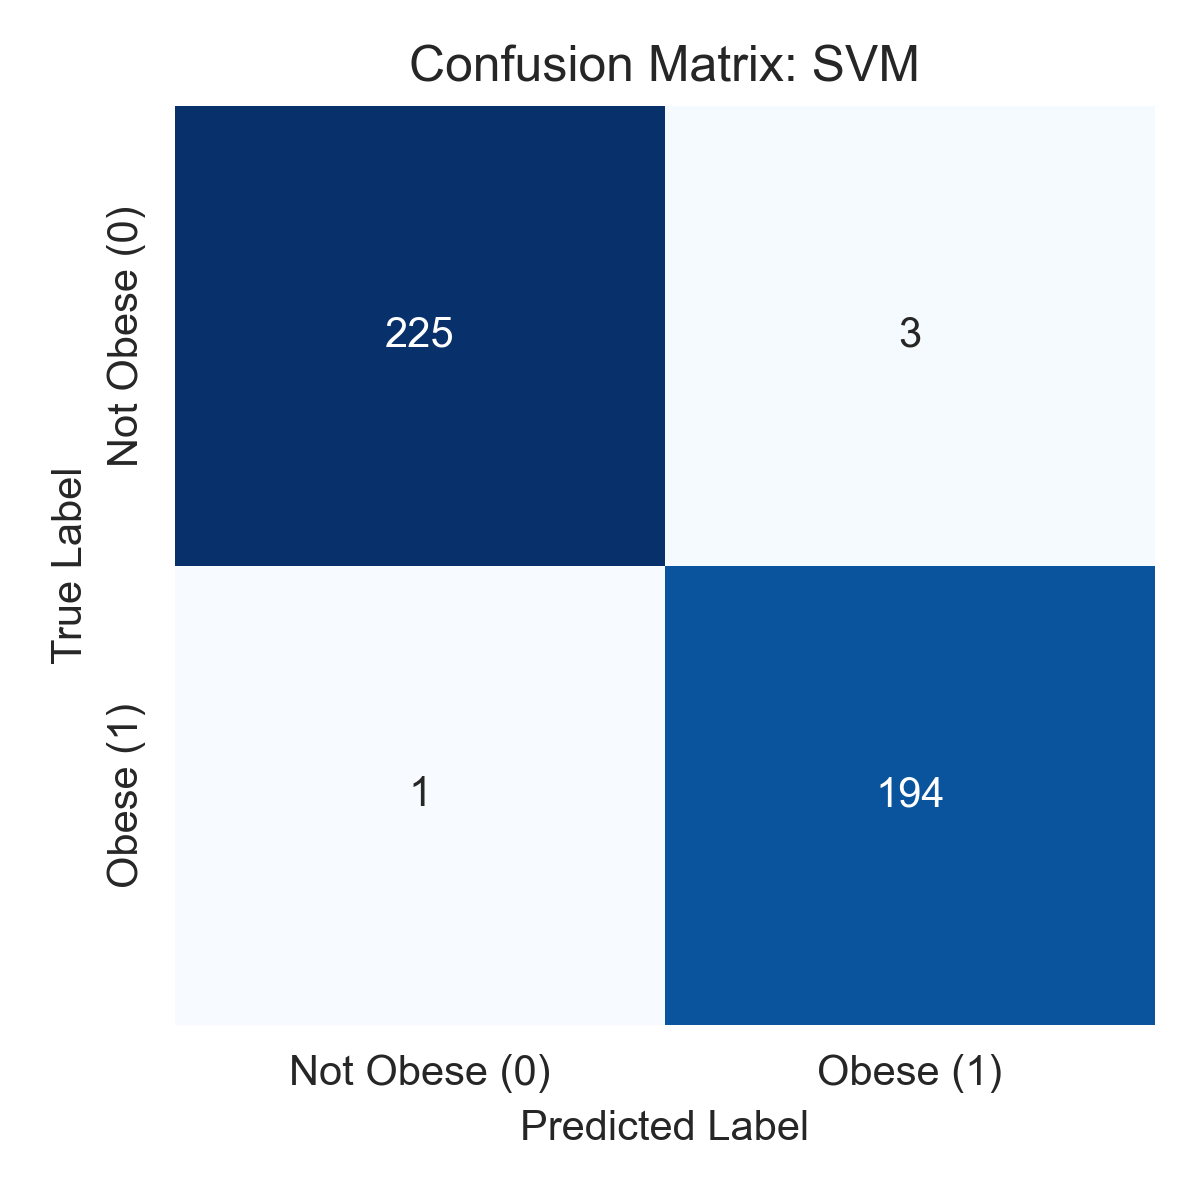
\includegraphics[width=\linewidth]{svm_confusion.png}
    \caption{SVM Confusion Matrix (with weight)}
\end{minipage}
\hspace{0.04\textwidth}
\begin{minipage}{0.35\textwidth}
    \centering
    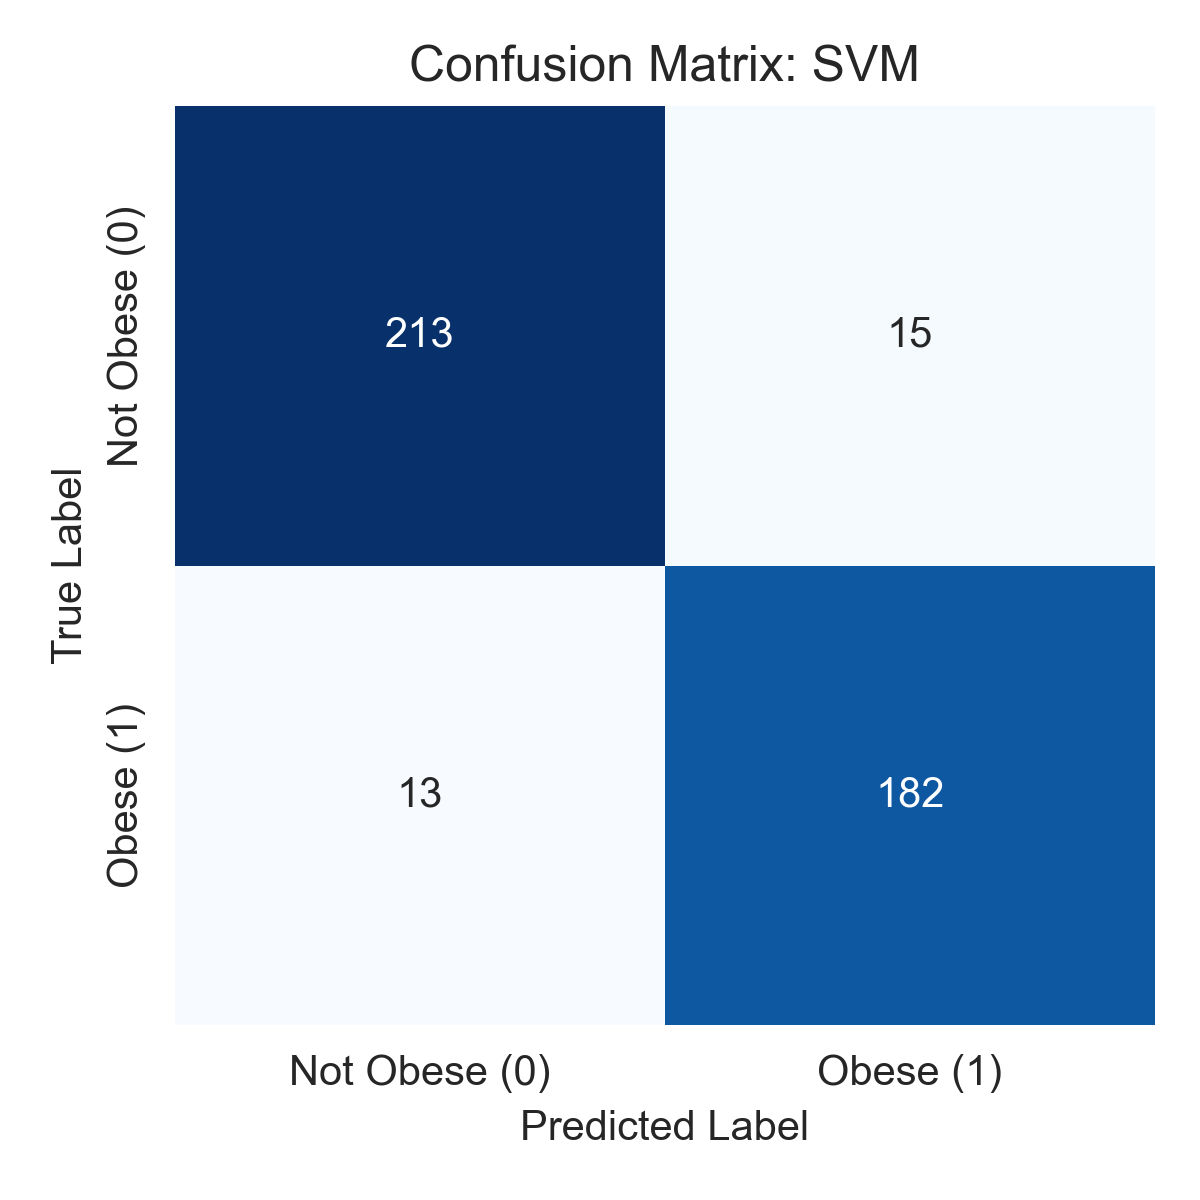
\includegraphics[width=\linewidth]{svm_confusion_withoutWeight.png}
    \caption{SVM Confusion Matrix (without weight)}
\end{minipage}
\label{fig:SVM_comparison}
\end{figure}

Like several other models in this project, SVM seems to have higher balanced accuracies on the testing data compared to the cross-validated set. It seems to classify each category equally in both variants of the analysis. It has fairly high balanced accuracies for both versions of the analysis.

\textbf{Conclusions:}
Predictably, when weight was removed, all models performed consistently worse. Weight seemed to be a very significant variable in all models. Interestingly enough, despite its removal for the second analysis, the models still performed very well. Balanced accuracies were still relatively high, with the exception of LDA, which was 0.7630, a stark drop from 0.9766 for the same metric when weight is included. In the analysis with weight, all models performed astoundingly high, with the lowest being QDA with a balanced accuracy of 0.9024. the best model was logistic regression with an $L_1$ penalty, which is LASSO regression. The analysis without weight, on the other hand, found the most success using Gradient Boosting, which boasts a balanced accuracy at 0.9755. The confusion matrices for models in each analysis are promising--they don't seem to favor one class over another.

\section{Feature Importance}
After calculating the performance metrics and confusion matrices for each method, I also did permutation feature importance. Below is a graph describing which features were most important for each model for both the variation with and without the weight variable.

\begin{figure}[H]
\centering
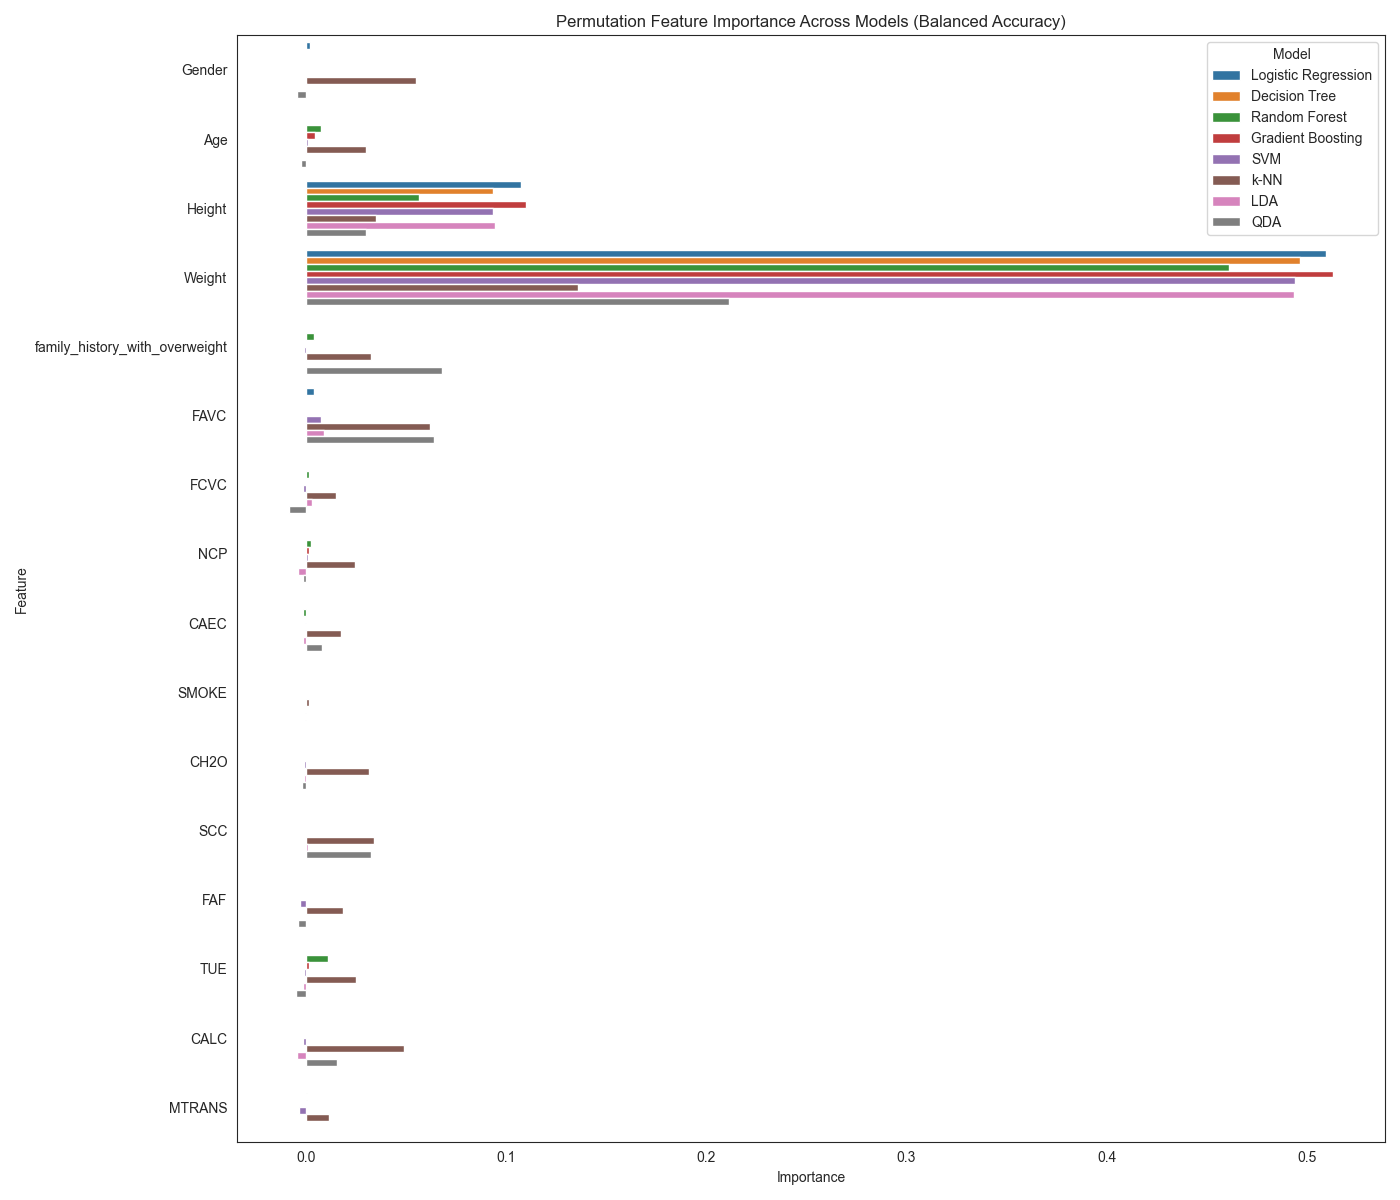
\includegraphics[width=0.95\textwidth]{Feature_Importance.png}
\caption{Permutation feature importance comparison with weight variable}
\label{fig:feature_importance}
\end{figure}

\begin{figure}[H]
\centering
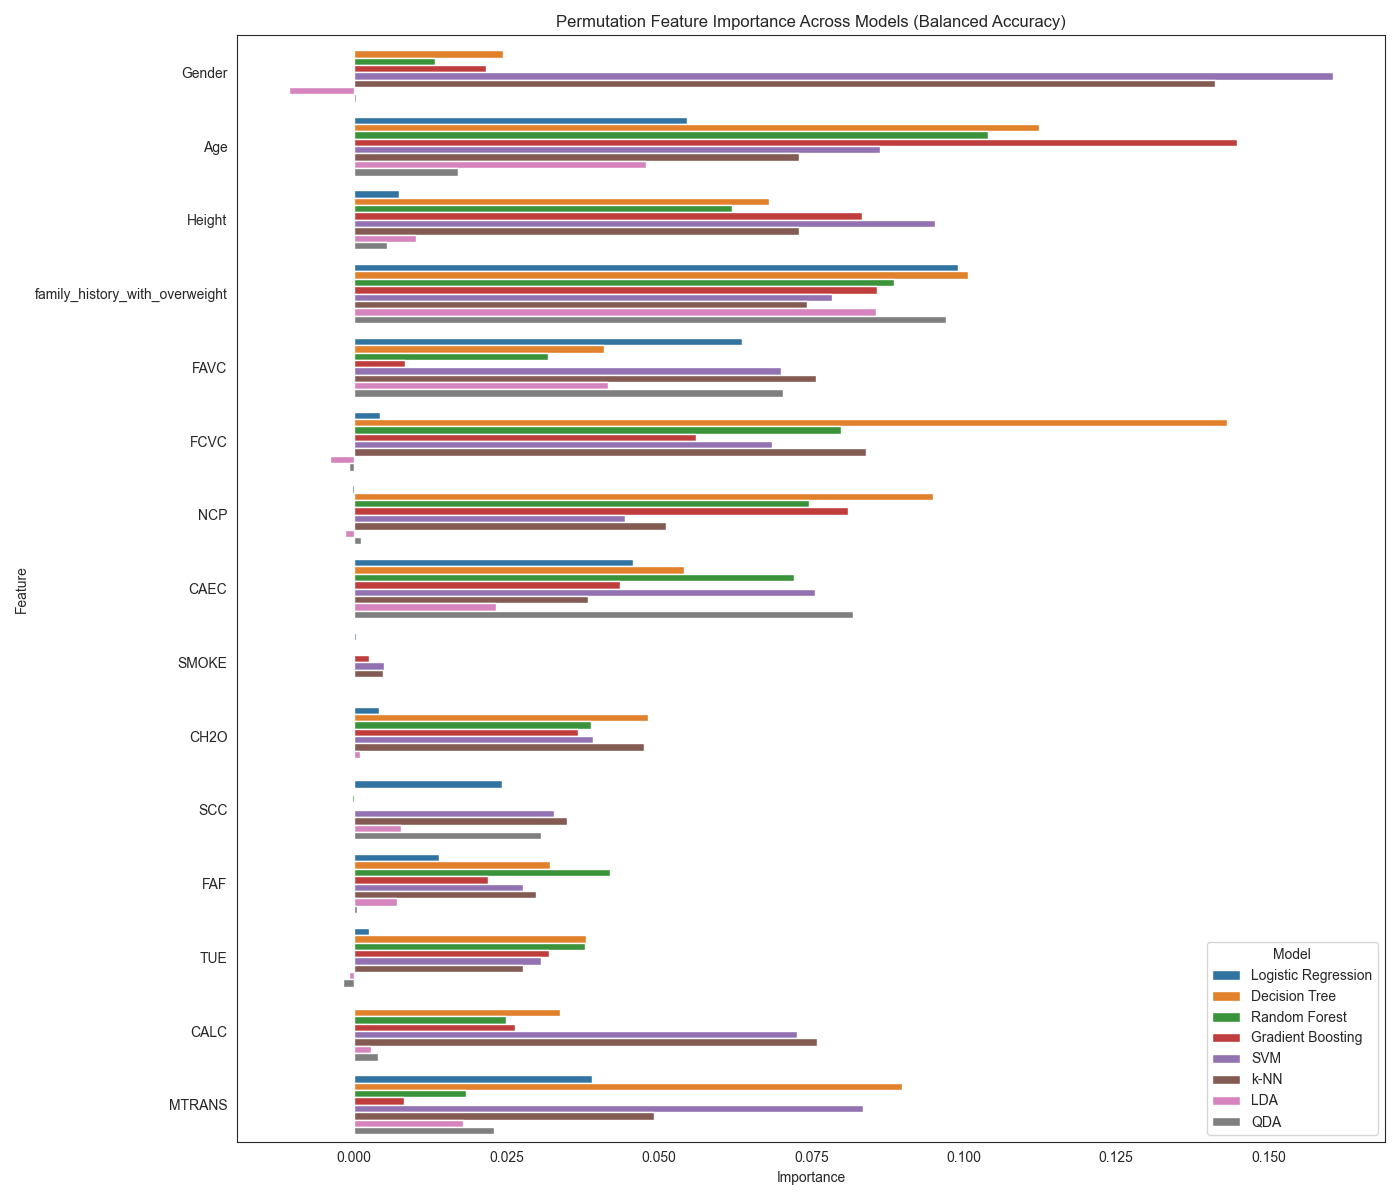
\includegraphics[width=0.95\textwidth]{Feature_Importance_noWeight.png}
\caption{Permutation feature importance comparison without weight variable}
\label{fig:feature_importance_withoutWeight}
\end{figure}

Unsurprisingly, in the variant with weight included, it is the variable of most importance in all models, though height also seemed to be significant. Of all the models, it seems k-NN seems to make the most use of all the variables to make a decision, followed by QDA. When the weight variable is removed, all features are used in a greater capacity. It is challenging to determine which feature is most important overall, as each model operates differently; however, age, height, and family history, FCVC (usually eats vegetables with meals), and CAEC (eating food between meals), seem like good candidates. Smoking seems to be the least relevant feature in all models.

\section{Final Thoughts}
While obesity remains an existing issue facing the global community, the data is clear--lifestyle factors have a strong effect on weight. After removing weight from the model, many of the most influential factors in determining obesity had to do with lifestyle and dietary choices, as seen in Figure \ref{fig:feature_importance_withoutWeight}. I was surprised with how high the balance accuracies were in this analysis, even with the weight variable removed. While I suspect there would be a distinction between the categories, I was not expecting it to be so clear across all model types. After considering the evaluation metrics, gradient boosting stands out as a clear winner. With its strong, accurate classification power and adaptability between the 2 variants of the analysis, it is the most effective approach for classifying obesity status. 


\newpage

\end{document}


